\documentclass[12pt,a4paper,openright,twoside]{report}

\usepackage{babel}
\usepackage[T1]{fontenc}

\usepackage{graphicx}
\graphicspath{ {img/} }

\usepackage{amsmath}
\usepackage{acronym}

% Geometry and microtype packages
\usepackage[
    a4paper,
    top=2cm,
    bottom=2cm,
    left=3cm,
    right=3cm,
    marginparwidth=1.75cm,
    inner=4cm,
    outer=2cm,
    heightrounded,
    ]{geometry}
\usepackage[protrusion=false, expansion=true]{microtype}

% Hyperref package for clickable links
\usepackage[hyphens]{url}
\usepackage{xurl}
\usepackage[
    breaklinks,
    pdfpagelabels,
    colorlinks=true,
    allcolors=black
]{hyperref}

% Bibliography management packages
\usepackage[style=ieee]{biblatex}
\DeclareFieldFormat{howpublished}{\url{#1}}
% \usepackage{csquotes}
\addbibresource{export.bib}
\setcounter{biburlnumpenalty}{9000}
\setcounter{biburllcpenalty}{9000} 
\setcounter{biburlucpenalty}{9000} 

% Font packages
\usepackage{listingsutf8}
\usepackage{pxfonts,fix-cm}
\usepackage{accsupp} % For non-copyable text (code numbering)
\newcommand{\noncopynumber}[1]{%
    \BeginAccSupp{method=escape,ActualText={}}%
    #1%
    \EndAccSupp{}%
}

\usepackage[table]{xcolor}
\definecolor{sviolet}{HTML}{6C71C4}
\definecolor{sbase1}{HTML}{93A1A1}
\definecolor{sblue}{HTML}{268BD2}
\definecolor{scyan}{HTML}{2AA198}
\definecolor{sbase00}{HTML}{657B83}
\lstset{
    inputencoding=utf8/latin1,
    language=Java, 
    columns=fullflexible,
    keepspaces=true,
    sensitive=true,
    aboveskip=\baselineskip,
    belowskip=\baselineskip,
    frame=lines,
    xleftmargin=\parindent,
    belowcaptionskip=1\baselineskip,
    basicstyle=\color{sbase00}\ttfamily,
    keywordstyle=\color{scyan},
    commentstyle=\color{sbase1},
    stringstyle=\color{sblue},
    numberstyle=\color{sviolet},
    identifierstyle=\color{sbase00},
    breaklines=true,
    showstringspaces=false,
    tabsize=2
}

\lstdefinestyle{mystyle}{
    basicstyle=\ttfamily\footnotesize,
    breaklines=true,
    columns=fullflexible,
    frame=single,
    captionpos=b,
    keepspaces=true,
    showspaces=false,
    showstringspaces=false,
    numberstyle=\tiny,
    numbers=left,
    stepnumber=1,
    numbersep=5pt
}

\usepackage{float}
\usepackage{parskip}
\usepackage[hypcap=true]{caption}
\usepackage{chngcntr}
\usepackage{listings, listings-rust}
\counterwithout{figure}{chapter}
\counterwithout{footnote}{chapter}
\counterwithout{table}{chapter}
\AtBeginDocument{
    \counterwithout{lstlisting}{chapter}
    \renewcommand{\thetable}{\arabic{table}}
    \renewcommand{\thelstlisting}{\arabic{lstlisting}}
}
\usepackage{awesomebox}
\setlength{\parskip}{6pt}
\setlength{\parindent}{0pt}

\usepackage{tikz}
\usepackage{changepage}
\usepackage{afterpage}

\definecolor{color_29791}{rgb}{0,0,0}
\definecolor{color_104998}{rgb}{0.290196,0.494118,0.733333}
\definecolor{AzulCeleste}{RGB}{31, 130, 192}


\usepackage{booktabs}
\usepackage{array}
\usepackage{tabularx}
\usepackage{todonotes}
\usepackage{siunitx}
\usepackage{multirow}

\lstset{
  inputencoding=utf8,
  extendedchars=true,
  literate=
    {á}{{\'a}}1 {é}{{\'e}}1 {í}{{\'i}}1 {ó}{{\'o}}1 {ú}{{\'u}}1
    {Á}{{\'A}}1 {É}{{\'E}}1 {Í}{{\'I}}1 {Ó}{{\'O}}1 {Ú}{{\'U}}1
    {ñ}{{\~n}}1 {Ñ}{{\~N}}1
}

% \usepackage{tocloft}

% \setlength{\cftbeforefigskip}{0pt}
% \setlength{\cftbeforetabskip}{0pt}


% \usepackage{etoolbox}

% \makeatletter
% \patchcmd{\l@figure}{\addvspace{10\p@}}{}{}{}
% \patchcmd{\l@table}{\addvspace{10\p@}}{}{}{}
% \makeatother

% \usepackage{latexsym} 
% \usepackage[none]{hyphenat}


\newcommand{\pfg}{Proyecto Fin de Grado }

\title{Outlier Detection System}
\author{Rubén Agustín González}

\raggedbottom

\begin{document}

\hypersetup{pageanchor=false}
\begin{titlepage}
    \thispagestyle{empty}
    \newgeometry{margin=0in}
\begin{tikzpicture}[overlay]\path(0pt,0pt);\end{tikzpicture}
\begin{picture}(-5,0)(2.5,0)
	\put(38.88,-35.76001){\fontsize{12}{1}\usefont{T1}{ptm}{m}{n}\selectfont\color{color_29791} }
	\put(38.88,-49.56){\fontsize{12}{1}\usefont{T1}{ptm}{m}{n}\selectfont\color{color_29791} }
	\put(38.88,-792.24){\fontsize{12}{1}\usefont{T1}{ptm}{m}{n}\selectfont\color{color_29791} }
	\put(178.5,-135.7297){
\includegraphics[width=252.1922pt,height=78.8pt]{latexImage_b33e2d3a1e077c187ed4eaa1710c29b2.png}}
\end{picture}
\begin{tikzpicture}[overlay]
	\path(0pt,0pt);
	\draw[color_104998,line width=15pt,line join=round]
	(38.8501pt, -33.38pt) -- (538.5001pt, -32.33002pt)
	;
	\draw[color_104998,line width=15pt,line join=round]
	(36.5501pt, -787.9316pt) -- (505.8501pt, -787.9316pt)
	;
	\draw[color_104998,line width=15pt,line join=round]
	(46.2502pt, -25.97992pt) -- (44.1502pt, -784.6299pt)
	;
	\draw[color_104998,line width=15pt,line join=round]
	(520.1499pt, -788.7799pt) -- (538.3999pt, -788.7799pt)
	;
\end{tikzpicture}

\tikz[remember picture,overlay]
	\node[opacity=0.3, inner sep=0pt] at ([xshift=2cm, yshift=-6cm]current page.center)
    {
\includegraphics[width=0.5\paperwidth, height=0.5\paperheight, keepaspectratio]{escudotrasparente.jpg}};



\vspace{7cm}
\begin{center}
	{\fontsize{20}{24} \textbf{PROYECTO FIN DE GRADO} } \\
	
\end{center}
\vspace{1,3cm}
%\begin{spacing}{2}
\begin{adjustwidth}{4cm}{3cm}
	{\setlength{\parskip}{0pt} \setlength{\parindent}{0pt}

{\fontsize{11}{13,2}
	{\textbf{TÍTULO:} Sistema de Detección de Anomalías para Proyecciones Multidimensionales en Tiempo Real}\vspace{19pt}
	
	{\textbf{AUTOR/A:} Rubén Agustín González }\vspace{19pt}
	
	{\textbf{TITULACIÓN:} Doble grado en Ingeniería electrónica de comunicaciones e Ingeniería telemática }\vspace{19pt}
	
	{\textbf{TUTOR/A:} Julián Nieto Valhondo} \vspace{19pt}
	
	{\textbf{DEPARTAMENTO:} DTE}\vspace{19pt}
	
	\hspace*{\fill}	{\textbf{VºBº TUTOR/A}  }\vspace{17pt}
	
	{\textbf{Miembros del Tribunal Calificador:}}\vspace{19pt}
	
	{\textbf{PRESIDENTE/A:} María Cristina Guerrero García}\vspace{19pt}
	
	{\textbf{TUTOR/A:} Julián Nieto Valhondo}\vspace{19pt}
	
	{\textbf{SECRETARIO/A:} Mariano Ruiz González}\vspace{19pt}
	
	{\textbf{Fecha de lectura:} Septiembre de 2025}\vspace{19pt}
	
	{\textbf{Calificación:} }\vspace{19pt}
	
	\hspace*{\fill}{\textbf{El Secretario/La Secretaria,}}\vspace{19pt}
}
}
\end{adjustwidth}

%\end{spacing}
\restoregeometry
\end{titlepage}
\pagenumbering{Roman}

\newpage
% Resumen (obligatorio)
\begin{abstract}
    Las disrupciones en plasmas de tokamak—colapso térmico rápido seguido de extinción de corriente, impulsados por inestabilidades magnetohidrodinámicas (MHD)—imponen riesgos termo-mecánicos y electromagnéticos que escalan de forma desfavorable con el tamaño del dispositivo. 
Anticipar estos eventos con el margen temporal suficiente es condición previa para la protección de la máquina y para habilitar una terminación o mitigación efectiva (p.\,ej., inyección masiva de gas o de \emph{pellets}). 
Este trabajo presenta un ensamble orientado por protocolo para la evaluación de disrupciones que integra modelos heterogéneos tras una interfaz \acs{HTTP}/OpenAPI unificada, habilitando componibilidad, versionado y despliegue entre lenguajes y \emph{runtimes}. 
El modelo de datos refleja el montaje experimental: siete diagnósticos síncronos muestreados cada 1\,ms desde el inicio de la descarga hasta su fin o disrupción. En su mayoría, el desbalance de clases proviene principalmente de la prevalencia de eventos (\(\sim\!6\%\) de descargas son disruptivas); la diferencia adicional de longitud entre descargas no disruptivas (\(\sim\!12\mathrm{k}\) muestras) y disruptivas (\(\sim\!7\mathrm{k}\) muestras) amplifica el desbalance cuando se entrena con ventanas de tamaño fijo. 
El preprocesado es causal en todos los modelos de predicción: las características por ventana y los normalizadores operan sin acceso a muestras futuras. Los descriptores informados por la física—medias por ventana, contenido espectral sin componente continua y cocientes simples que capturan la proximidad a límites operativos—preservan la interpretabilidad a la vez que enfatizan precursores relevantes para evitación y mitigación. 
El ensamble admite tanto evaluación con ventanas fijas como alerta temprana deslizante en flujo, exponiendo puntuaciones calibradas y justificaciones a nivel de ventana para sustentar una lógica de decisión conservadora en el orquestador. 
La generalización se trata como un riesgo de primer orden: la bibliografía reporta la pobre extrapolación de predictores específicos de dispositivo y subraya la necesidad de bases de datos multi-máquina, bien normalizadas y adimensionales para su aplicabilidad en máquinas de siguiente paso. 
En consecuencia, el flujo de trabajo se centra en validación entre campañas, diagnóstico de desplazamiento de covariables y la incorporación opcional de restricciones físicas para mejorar la transportabilidad, ofreciendo una base reproducible para investigación en predicción de disrupciones y un camino práctico hacia la integración en tiempo real en dispositivos actuales y, con adaptación de dominio, en máquinas de mayor tamaño como \ac{ITER}.

\end{abstract}
\renewcommand{\abstractname}{Abstract}
\newpage
% Abstract (obligatorio)
\vspace{10cm}
\begin{abstract}
    Disruptions in tokamak plasmas—rapid losses of thermal energy followed by current quench driven by \ac{MHD} instabilities—pose severe thermo-mechanical and electromagnetic risks that scale unfavorably with device size. Anticipating these events with sufficient lead time is a prerequisite for machine protection and for enabling effective termination or mitigation (e.g., massive gas or pellet injection). 
This work presents a protocol-driven ensemble for disruption assessment that integrates heterogeneous models behind a unified \acs{HTTP}/OpenAPI interface, enabling composability, versioning, and deployment across languages and runtimes. 
The data model mirrors the experimental setup: seven synchronous diagnostics sampled every 1\,ms from shot start until termination or disruption. Crucially, class imbalance arises primarily from discharge prevalence (\(\sim\!6\%\) of shots are disruptive); the additional length disparity between non-disruptive (\(\sim\!12\mathrm{k}\) samples) and disruptive (\(\sim\!7\mathrm{k}\) samples) shots further amplifies imbalance when training on fixed-size windows. 
Preprocessing is causal in every prediction model: windowed features and normalizers operate without access to future samples.
Physics-informed descriptors—mean values per window and DC-free spectral content, complemented by inter-signal ratios such as radiated-to-input power fraction, Greenwald fraction, and inductance/current normalizations—capture relevant precursors while preserving interpretability. 
The ensemble supports both fixed-length evaluation and rolling early-warning on streams, exposing calibrated scores and justifications at the window level to facilitate conservative decision logic in the orchestrator (thresholding and refractory policies). 
Generalization is treated as a first-class concern: the literature highlights the poor extrapolation of device-specific predictors and the need for well-normalized multi-machine, dimensionless datasets for next-step applicability. 
Accordingly, the workflow centers on cross-campaign validation, diagnostics of covariate shift, and optional physics constraints to improve transportability. 
The resulting toolkit delivers a reproducible baseline for disruption prediction research and a practical path toward real-time integration, while explicitly acknowledging the limits of training on historical data from a single tokamak and the consequent need for domain adaptation before deployment on larger devices such as \ac{ITER}.

\end{abstract}

\chapter*{Agradecimientos}


\hypersetup{pageanchor=false}
\hypersetup{linkcolor=black}
\tableofcontents

\listoffigures
\listoftables
\lstlistoflistings
\listoftodos

\chapter*{Acronyms} \label{sec:acronym}

% Acronyms list: Add to espanso configuration for automatic replacement
\begin{acronym}[EURATOM]
    \acro{APODIS}{Advanced Predictor of Disruptions}
    \acro{CIEMAT}{\textit{Centro de Investigaciones Energéticas, Medioambientales y Tecnológicas}}
    \acro{CNN}{Convolutional Neural Network}
    \acro{EAST}{Experimental Advanced Superconducting Tokamak}
    \acro{EIF}{Extended Isolation Forest}
    \acro{EURATOM}{European Atomic Energy Community}
    \acro{FPGA}{Field-Programmable Gate Array}
    \acro{FFT}{Fast Fourier Transform}
    \acro{GBDT}{Gradient-Boosted Decision Tree}
    \acro{GPU}{Graphics Processing Unit}
    % \acro{I2A2}{\textit{Investigación en Instrumentación y Acústica Aplicada}}
    \acro{HPC}{High-Performance Computer}
    \acro{HTTP}{Hypertext Transfer Protocol}
    \acro{IForest}{Isolation Forest}
    \acro{ITER}{International Thermonuclear Experimental Reactor}
    \acro{JET}{Joint European Torus}
    \acro{LSTM}{Long Short-Term Memory}
    \acro{MHD}{Magneto-hydrodynamic}
    \acro{ML}{Machine Learning}
    \acro{npm}{Node Package Manager}
    \acro{OC-SVM}{One-Class SVM}
    \acro{PTP}{Precision Time Protocol}
    \acro{SDG}{Sustainable Development Goals}
    \acro{RMS}{Root Mean Square}
    \acro{STFT}{Short-Time Fourier Transform}
    \acro{SVM}{Support Vector Machine}
    \acro{UN}{United Nations}
    % \acro{YAML}{YAML Ain't Markup Language}
\end{acronym}



% Contenidos
\pagenumbering{arabic}

\chapter{Introduction} \label{sec:cap1}

\section{Context and Motivation}

This project has been developed as a final project for the Electronic Engineering degree at the investigation group \ac{I2A2} and belongs to the \ac{ITER} project. The main goal is to create an outlier detection system that can be used to monitor the performance of the \ac{ITER} reactor, ensuring its safe and efficient operation.


\chapter{State of the Art} \label{sec:cap2}

\section{Introduction to Nuclear Fusion}

Nuclear fusion is the process in which two light atomic nuclei combine to form a heavier nucleus, releasing a substantial amount of energy. This is the same reaction that powers the Sun and other stars, making it a potential source of clean, virtually limitless energy for humanity.

The primary fuels for fusion are hydrogen isotopes such as deuterium and tritium. Their fusion produces helium and a high-energy neutron, releasing energy mainly as the kinetic energy of the neutron and, to a lesser extent, electromagnetic radiation.

Achieving controlled fusion on Earth requires overcoming the electrostatic repulsion between positively charged nuclei, which demands extremely high temperatures (on the order of tens of millions of kelvin) and sufficient pressure. These conditions can be achieved through magnetic confinement — in devices known as tokamaks — or through inertial confinement using high-power lasers.


\section{Nuclear Fusion on \acs{ITER} and \acs{JET}}

The \ac{ITER} project is an international collaboration designed to demonstrate the feasibility of nuclear fusion as a large-scale, carbon-free energy source. Under construction in Cadarache, France, ITER involves 35 countries, including members of the European Union, the United States, China, India, Japan, Russia, and South Korea. It will house the world's largest tokamak, using magnetic confinement to heat plasma to fusion conditions.\ \ac{ITER} is designed to produce ten times more fusion power than the power used to heat the plasma, representing a major step toward commercial fusion energy.

The \ac{JET} was, until December 2023, the largest operational tokamak in the world. Located in Culham, UK, it played a key role in advancing fusion research, testing plasma scenarios, and validating technologies for \ac{ITER} and future reactors. Following its final deuterium-tritium experiments, JET ceased plasma operations, and the largest operational tokamak is now JT-60SA in Japan \autocite{JT60SACertifiedWorlds2024,FusionenergyQuestMakes2024}.

The \ac{CIEMAT} is Spain's representative in \ac{EURATOM}'s fusion program, which includes participation in \ac{JET} and \ac{ITER}. For this project, \ac{CIEMAT} has provided experimental data from \ac{JET}, consisting of recorded plasma discharges.

\section{Discharges and Disruptions}

A \textit{Discharge} is a plasma operation in the tokamak, where the plasma is created and maintained for a certain period. Each discharge is characterized by various parameters, such as plasma current, inductance, density, radiated power or input power. When these parameters deviate from their expected values, it can indicate potential issues or anomalies in the reactor's operation.

A \textit{Disruption} is an event that occurs when the plasma becomes unstable and loses confinement, leading to a rapid cooling of the plasma (\textit{termal quench}) followed by a rapid loss of plasma current (\textit{current quench}). For this project, discharges are classified as either disruptive or non-disruptive.

A \textit{Campaign} is a set of discharges that are analyzed together. For this project, there are three campaigns available, each containing a different number of discharges. The available data for the project is summarized in \autoref{tab:campaigns}. This data is collected from the \ac{JET} tokamak and stored in text files for later analysis.

\begin{table}[htbp]
    \centering
    \caption{Available data for the project}
    \begin{tabular}{
        l
        S[table-format=3]  % Number of discharges
        S[table-format=2]  % Disruptive
        S[table-format=3]  % Non Disruptive
        S[table-format=1.2]@{\,}  % Rate
    }
    \toprule
    \textbf{Campaign} & \textbf{Discharges} & \textbf{Disruptive} & \textbf{Non--Disruptive} & \textbf{Disruption Rate} \\
    \midrule
    C23 & 522 & 32 & 490 & 6.13 \ \% \\
    C24 & 388 & 26 & 362 & 6.70 \ \% \\
    C25 & 611 & 41 & 570 & 6.71 \ \% \\
    \bottomrule
    \end{tabular}
    \label{tab:campaigns}
\end{table}

A visual representation of the plasma current on several discharges is shown in \autoref{fig:plasma-current}. This figure illustrates the singular bathtub shape of non-disruptive discharges, whereas disruptive discharges show a more erratic pattern.

\begin{figure}[H]
    \centering
    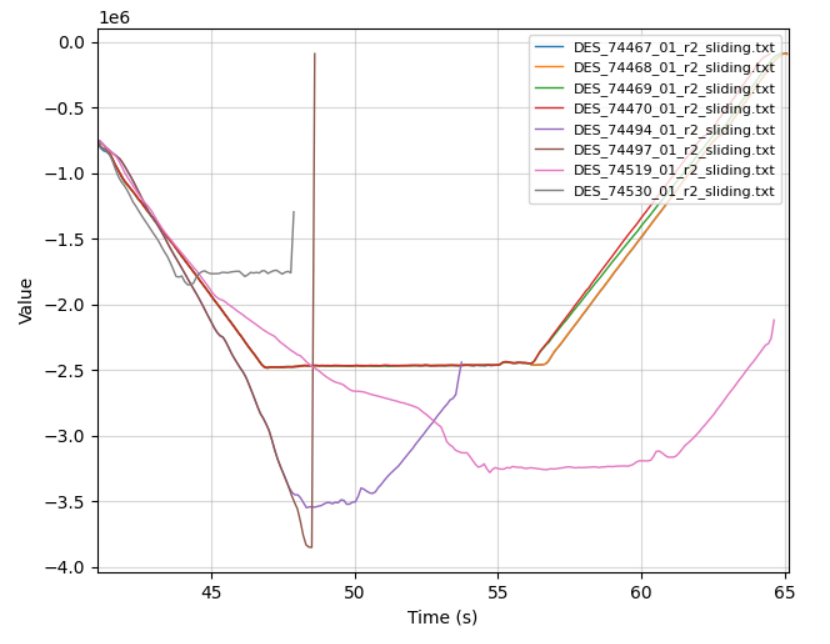
\includegraphics[width=0.8\textwidth]{plasma-current.png}
    \caption{Plasma current on disruptive and non-disruptive discharges}
    \label{fig:plasma-current}
\end{figure}

\section{Anomaly Detection in Nuclear Fusion}

Anomaly detection in nuclear fusion is crucial for ensuring the safe and efficient operation of reactors like \ac{ITER}. The complexity of the plasma behavior and the multitude of parameters involved make it challenging to monitor and control the system effectively. Anomalies can lead to disruptions, which can damage the reactor components and affect the overall performance.

To address this challenge, various machine learning techniques have been applied to analyze the data generated during discharges. These techniques aim to identify patterns and deviations in the data that may indicate potential anomalies. An early detection of these anomalies is essential to prevent disruptions and ensure the stability of the plasma, using gas injection to stop the nuclear fusion reaction before it causes damage to the reactor.

There are two main approaches to anomaly detection in nuclear fusion: neural-network-based models and physical models. Neural networks are trained on historical data to learn the patterns of normal operation, and then used to detect anomalies in real-time data. Physical models, on the other hand, are based on the physics of the plasma and are used to predict the behavior of the plasma under different conditions.

Neural networks have shown promising results in detecting anomalies, but some studies have raised concerns about their reliability and generalization capabilities.\ \textcite[p.~S188]{henderChapter3MHD2007} identify intrinsic limitations of neural-network disruption predictors—most notably, intrinsically poor extrapolation when entering new or expanded operating regimes—and argue that methods intended for a next-step device must rely on a high-quality, well-normalized, multi-machine, dimensionless database. In the same vein, \textcite[p.~2]{murariControlOrientedStrategy2024} report that device-specific ML predictors are typically limited to their tokamak of origin and that their extrapolation to larger, future devices (e.g., \ac{ITER}) is doubtful, owing to differences in scale (stored energy, $I_p$, $\beta_N$), materials and wall conditions, actuator authority, and disruption phenomenology. Taken together, these results imply that models trained solely on historical data from present machines cannot be trusted \emph{a priori} on ITER without cross-machine validation, physics-informed inductive biases, domain adaptation to covariate/concept shift, and calibrated uncertainty quantification.



\subsection{Introduction to \acs{APODIS}}

\ac{CIEMAT} uses the \ac{APODIS} algorithm, which is based on a \ac{SVM} model trained on historical discharge data.\ \ac{SVM} is a machine learning algorithm whose goal is to find the optimal hyperplane that separates the data into different classes \autocite{6524743}. Further explanation of \ac{SVM} is provided in \autoref{sec:svm}.

The model is designed to classify discharges as normal or anomalous based on the input parameters. The training process involves using labeled data, where each discharge is categorized as either normal or anomalous.

The \ac{APODIS} algorithm uses the signals listed in \autoref{tab:apodis-signals}.

\begin{table}[htbp]
  \centering
  \caption{List of signals analyzed in the \ac{APODIS} algorithm}
  \label{tab:apodis-signals}
  \begin{tabular}{@{}l c@{}}
    \toprule
    \textbf{Signal Name} & \textbf{Units} \\
    \midrule
    (1) Plasma Current                             & \si{A} \ \ \  \\
    (2) Mode Lock Amplitude                        & \si{T} \ \ \  \\
    (3) Plasma internal inductance                 &             \\ % adimensional
    (4) Plasma density                             & \si{\per\cubic\metre} \\
    (5) Stored diamagnetic energy time derivative  & \si{W} \ \ \  \\
    (6) Radiated Power                             & \si{W} \ \ \  \\
    (7) Total Input power                          & \si{W} \ \ \  \\
    \bottomrule
  \end{tabular}
\end{table}

The algorithm divides the discharge into windows of 16 milliseconds, and extracts the mean value and the \ac{FFT} of each window. On the prediction phase, the model receives a data stream, and fills a buffer to create a window. Then, it extracts the same features as in the training phase, and predicts the category of this window. If the model predicts an anomalous window, the discharge is classified as anomalous.

The \ac{APODIS} algorithm is a highly effective tool for detecting anomalies. The features extracted from the discharge data allow the model to capture the dynamics of the plasma behavior, that clearly differ between disruptive and non-disruptive discharges, as shown in \autoref{fig:psd}, where x-axis represents the frequency in Hz, and the y-axis represents the power spectral density in dB. The blue line represents the mean value for non-disruptive discharges, and the orange line represents the mean value for disruptive discharges. Scattered points represent the individual values for each disruptive discharge on the last window before the disruption.

Effectiveness of the \ac{APODIS} features are explained due to their physical meaning. On the one hand, the mean value of the signals captures the average behavior of the plasma during the discharge, which is useful for detecting anomalies that affect the overall plasma behavior. On the other hand, the \ac{FFT} captures the global growth of plasma fluctuations, which is associated to \ac{MHD} instabilities \autocite{liMHDInstabilityDynamics2023}.

\begin{figure}[htbp]
  \begin{subfigure}{.5\textwidth}
    \centering
    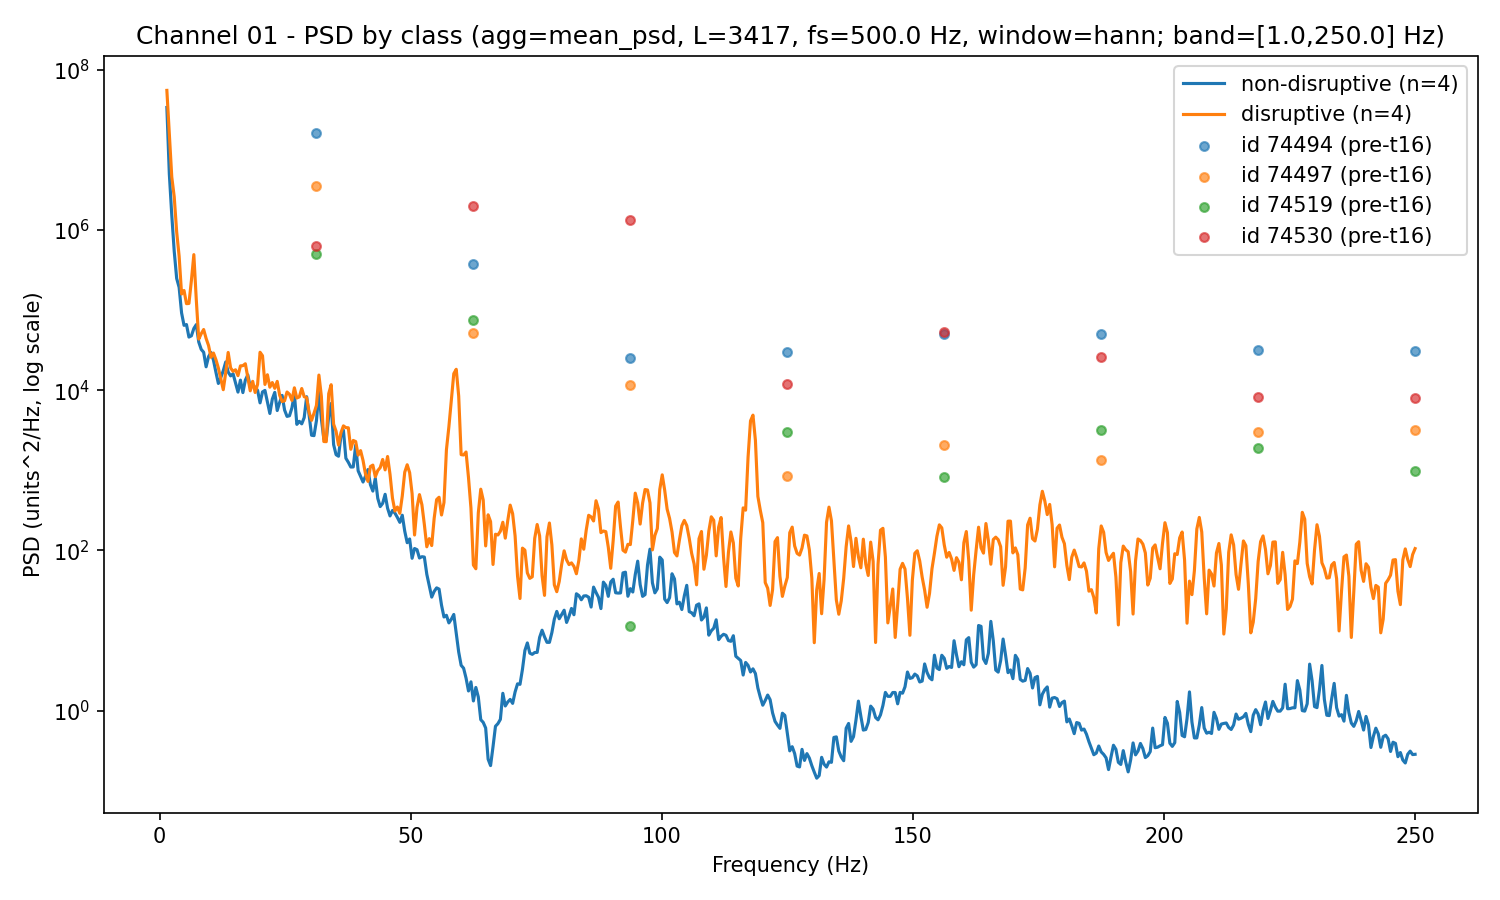
\includegraphics[width=.8\linewidth]{psd/psd_channel_01_mean_psd_band_1_250.png}
    \caption{Plasma Current}
    \label{fig:psd_channel_01_mean_psd_band_1_250}
  \end{subfigure}
  \begin{subfigure}{.5\textwidth}
    \centering
    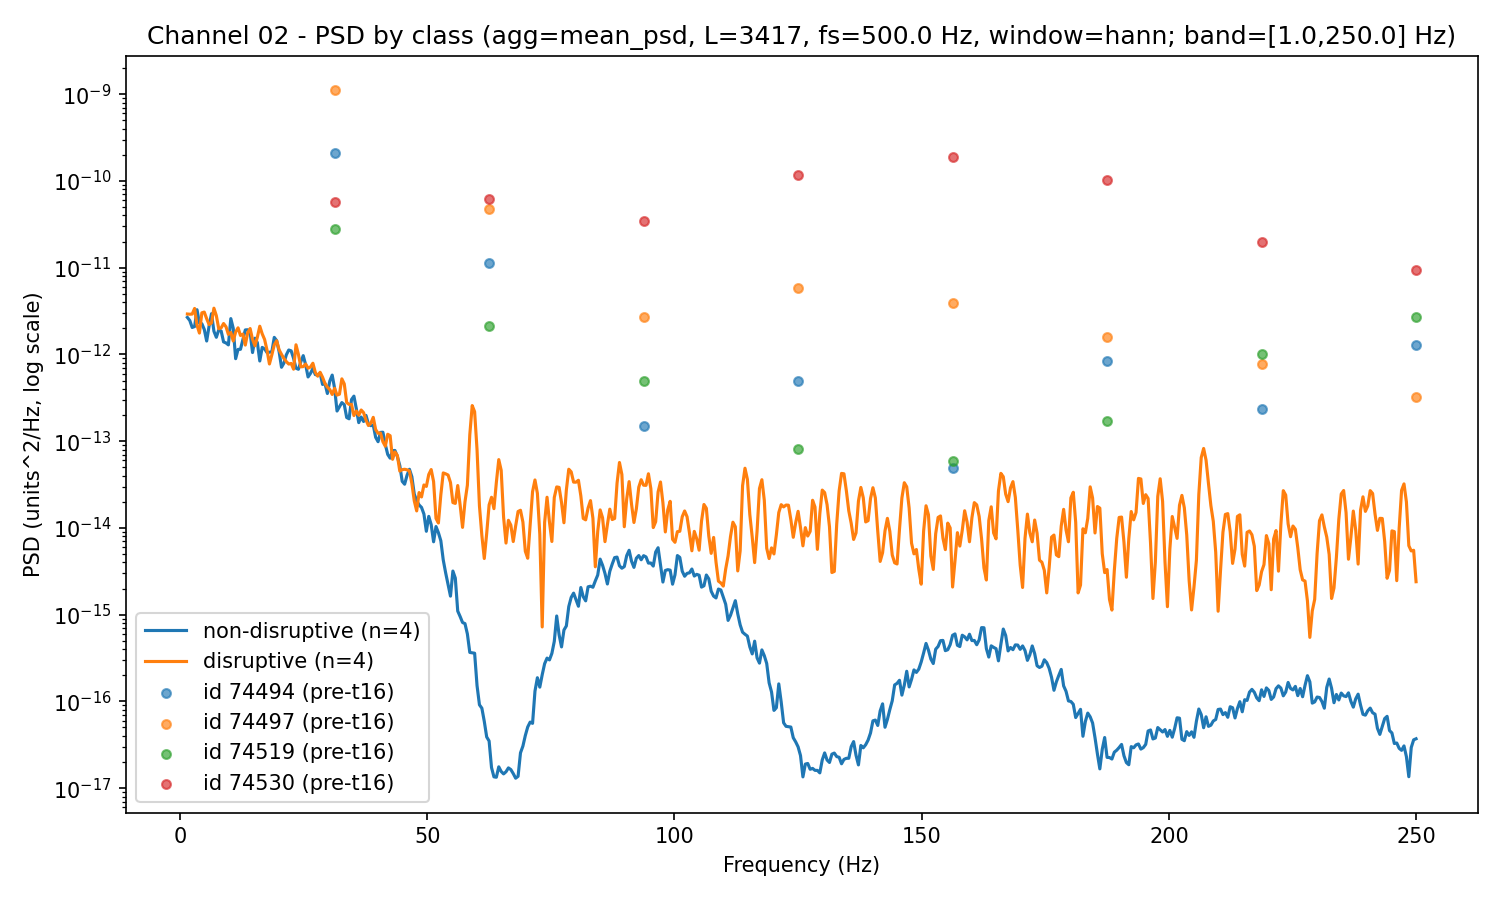
\includegraphics[width=.8\linewidth]{psd/psd_channel_02_mean_psd_band_1_250.png}
    \caption{Mode Lock Amplitude}
    \label{fig:psd_channel_02_mean_psd_band_1_250}
  \end{subfigure}
  \begin{subfigure}{.5\textwidth}
    \centering
    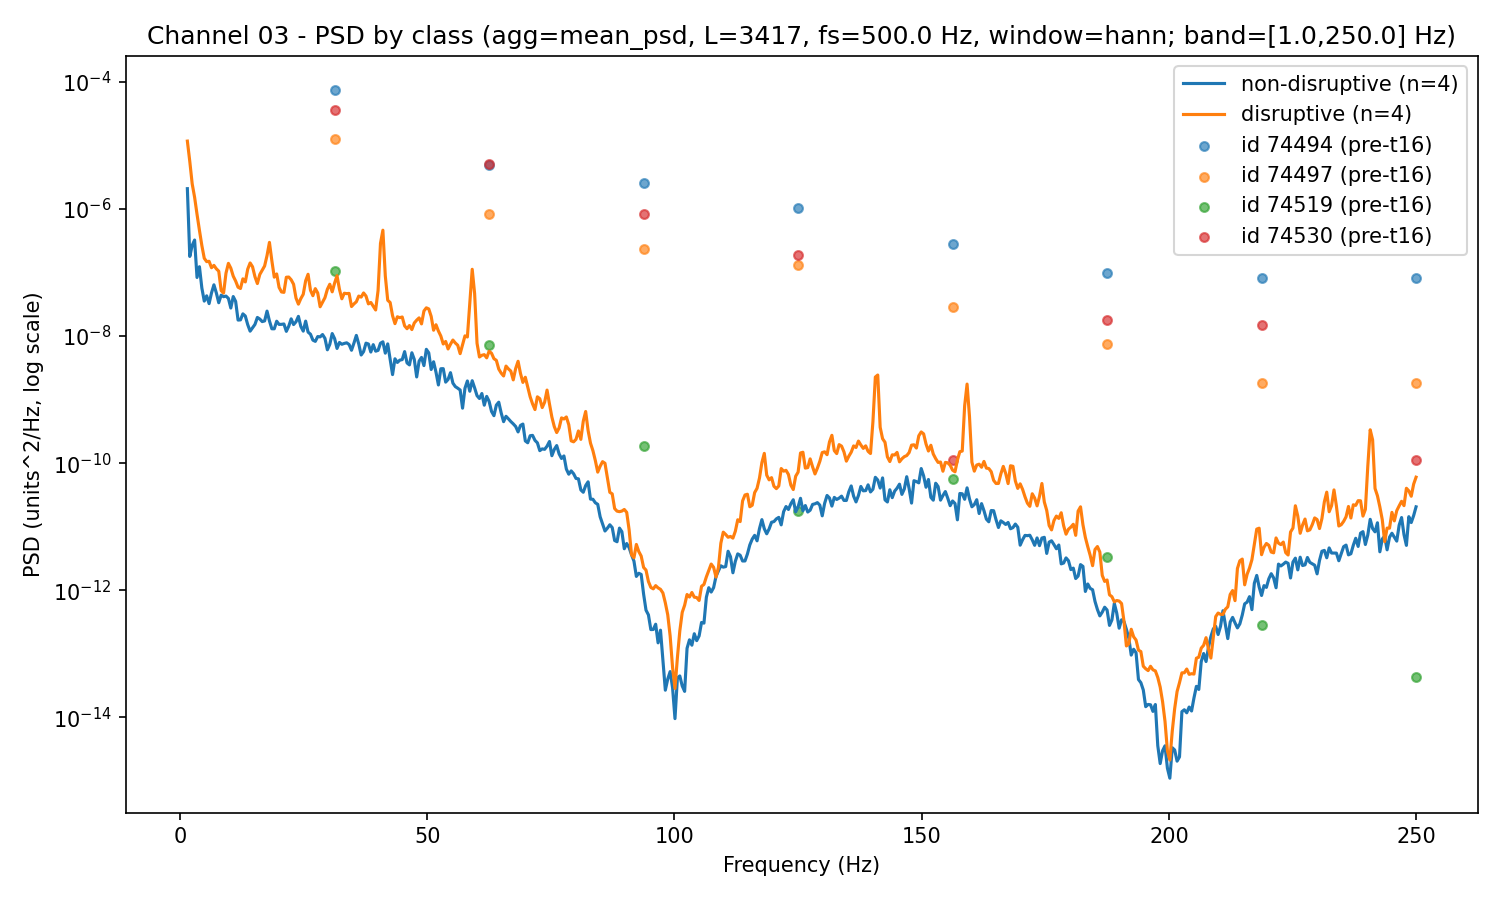
\includegraphics[width=.8\linewidth]{psd/psd_channel_03_mean_psd_band_1_250.png}
    \caption{Plasma internal inductance}
    \label{fig:psd_channel_03_mean_psd_band_1_250}
  \end{subfigure}
  \begin{subfigure}{.5\textwidth}
    \centering
    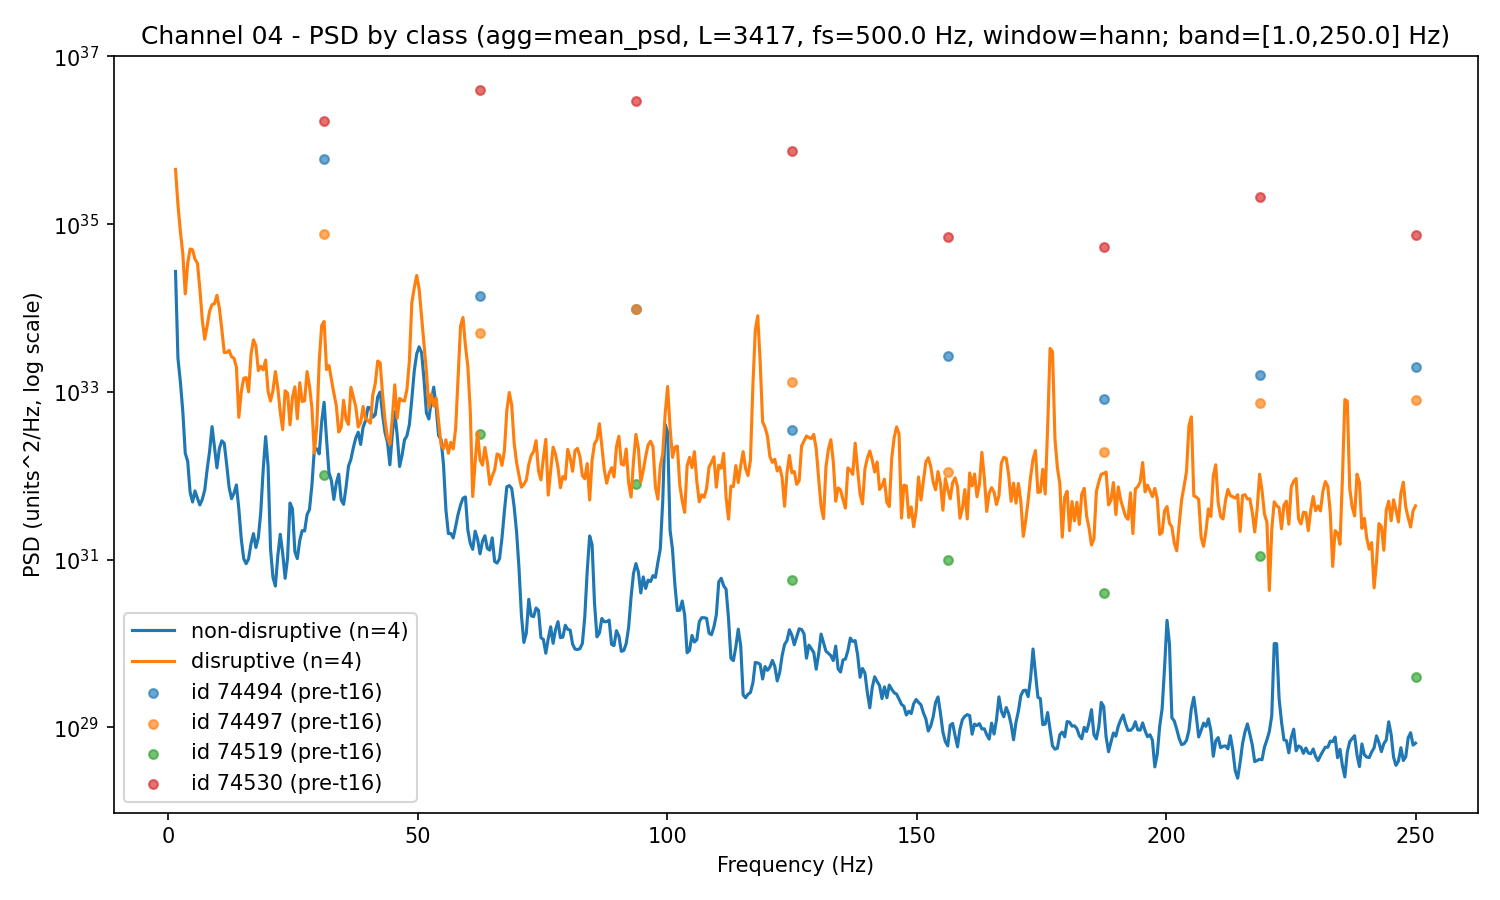
\includegraphics[width=.8\linewidth]{psd/psd_channel_04_mean_psd_band_1_250.png}
    \caption{Plasma density}
    \label{fig:psd_channel_04_mean_psd_band_1_250}
  \end{subfigure}
  \begin{subfigure}{.5\textwidth}
    \centering
    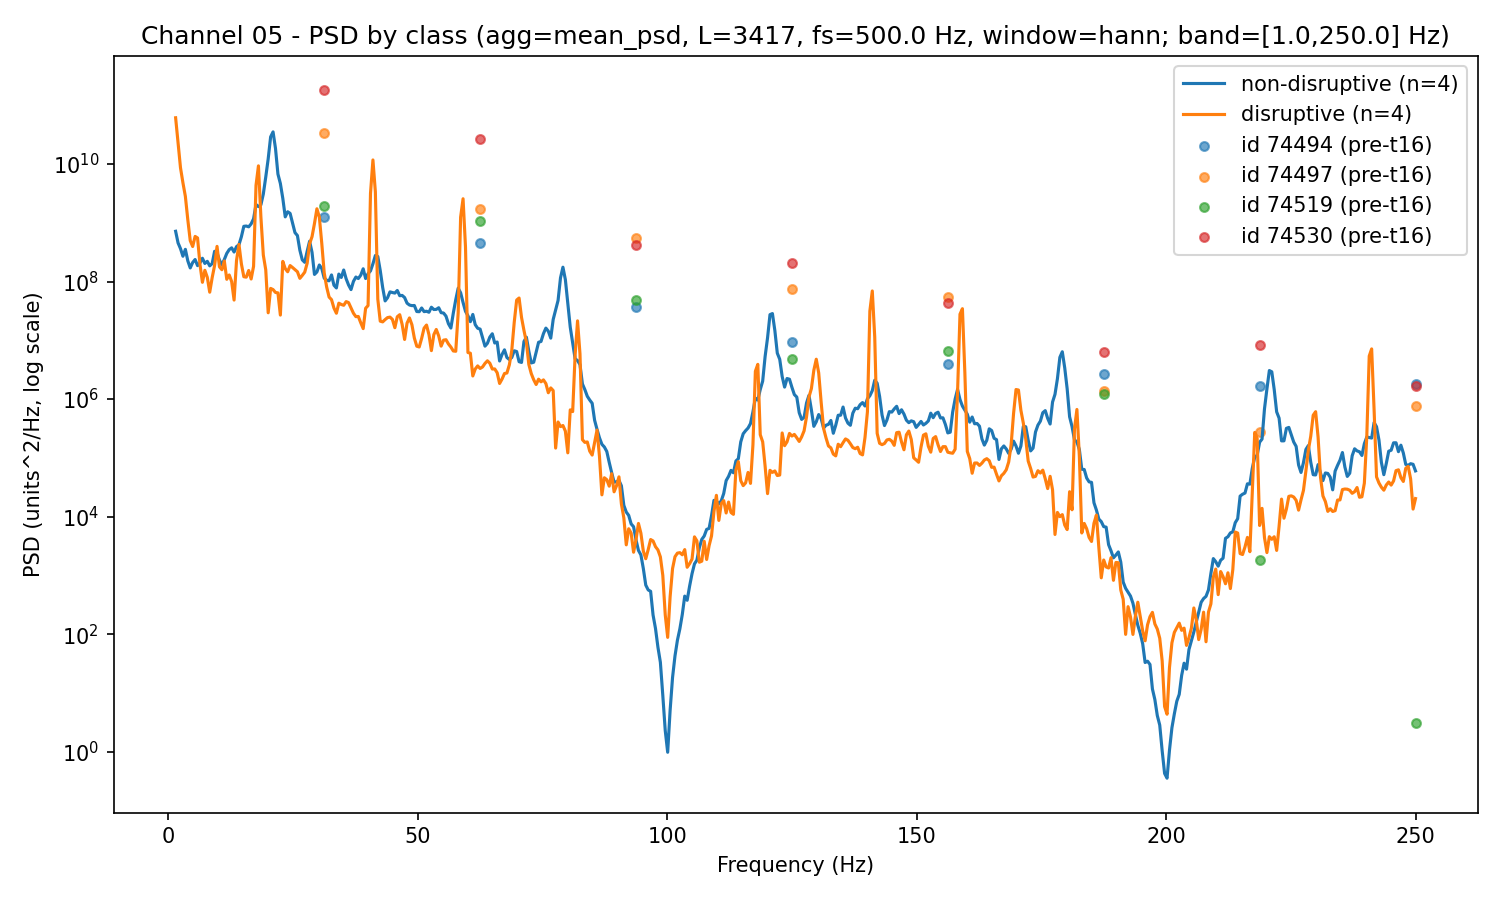
\includegraphics[width=.8\linewidth]{psd/psd_channel_05_mean_psd_band_1_250.png}
    \caption{Stored diamagnetic energy time derivative}
    \label{fig:psd_channel_05_mean_psd_band_1_250}
  \end{subfigure}
  \begin{subfigure}{.5\textwidth}
    \centering
    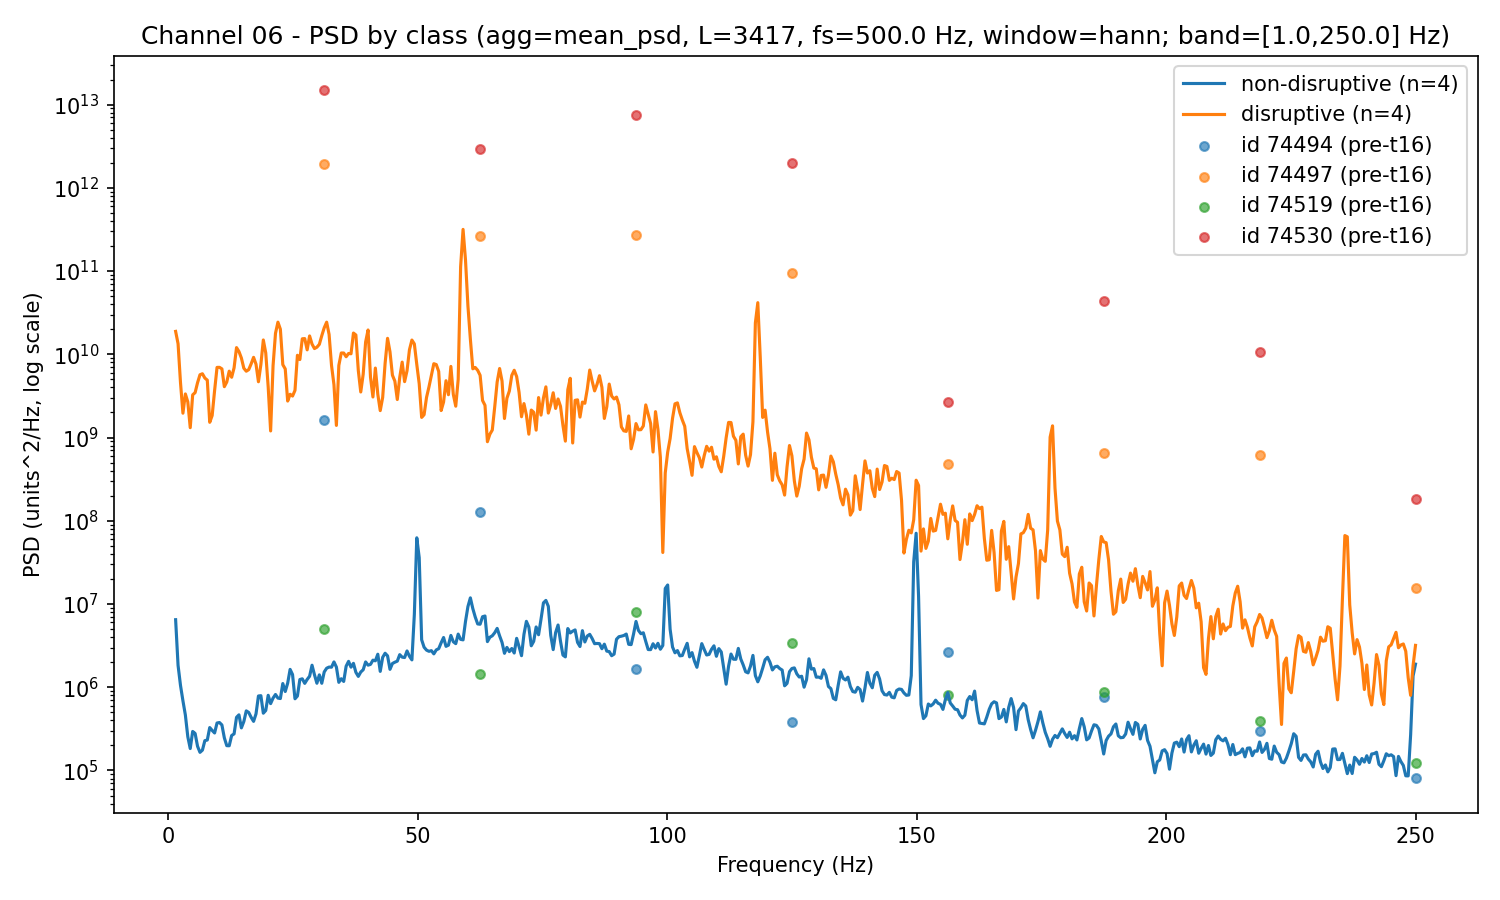
\includegraphics[width=.8\linewidth]{psd/psd_channel_06_mean_psd_band_1_250.png}
    \caption{Radiated Power}
    \label{fig:psd_channel_06_mean_psd_band_1_250}
  \end{subfigure}
  \begin{subfigure}{\textwidth}
    \centering
    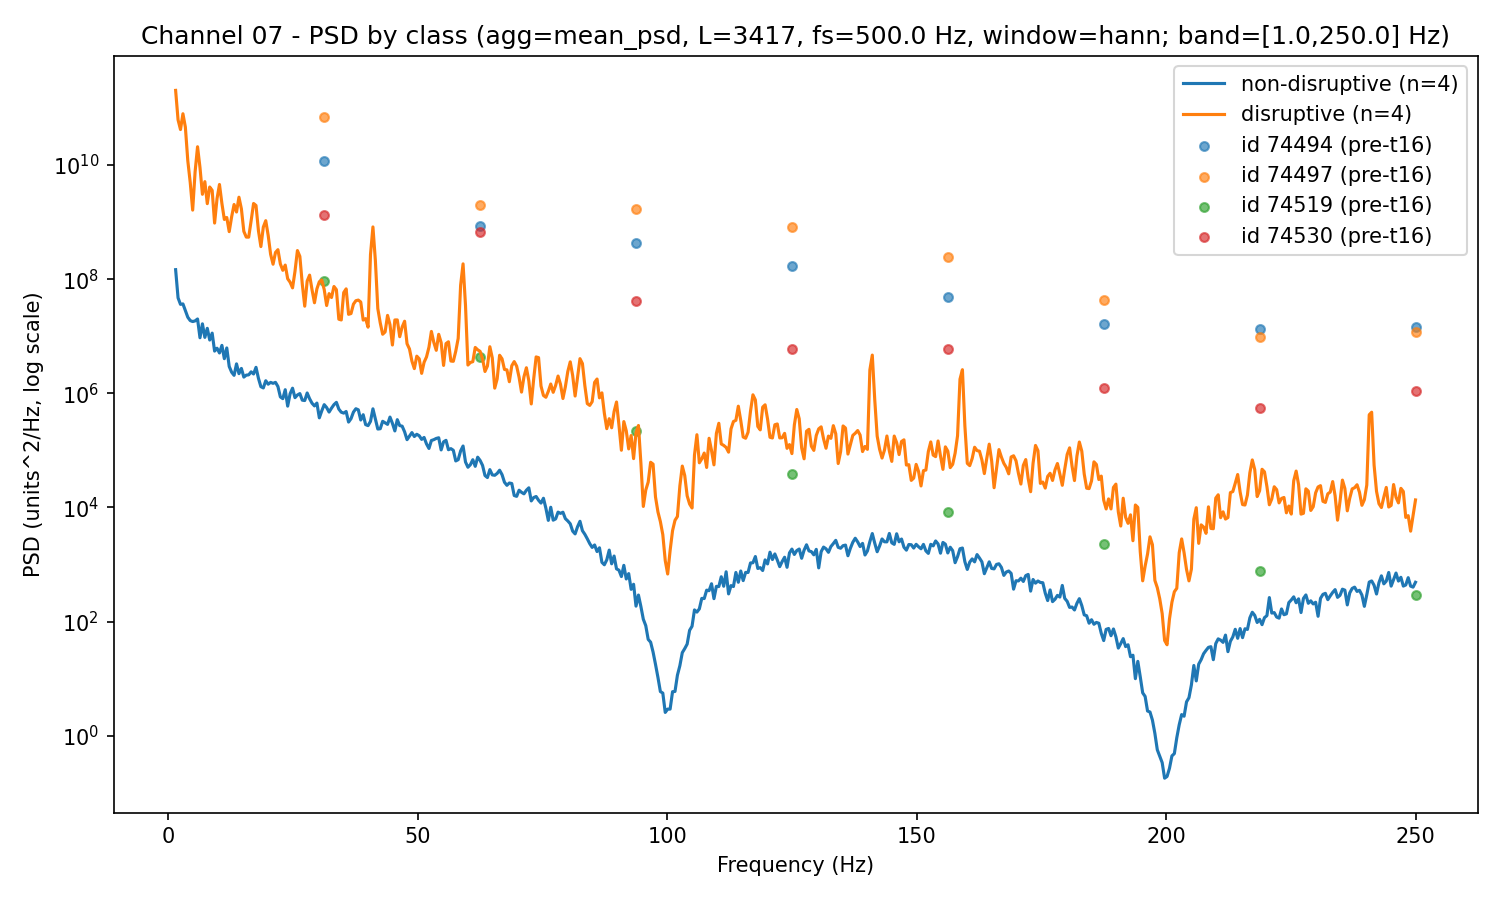
\includegraphics[width=.6\linewidth]{psd/psd_channel_07_mean_psd_band_1_250.png}
    \caption{Total Input power}
    \label{fig:psd_channel_07_mean_psd_band_1_250}
  \end{subfigure}
  \caption{Power Spectral Density of the signals used in the \ac{APODIS} algorithm}
  \label{fig:psd}
\end{figure}

Even though, there are some limitations to this approach. First, a window-based approach does not take into account large temporal dependencies of the data. This means that the model may not be able to capture the dynamics of the plasma behavior over time. Second, \ac{SVM} models with non-linear kernels have a complexity between $O(n^2)$ and $O(n^3)$, where $n$ is the number of training samples. This means that the model may not be able to scale to large datasets \autocite{kekulawalaSupportVectorMachines2024}. Third, even though \ac{SVM} models do not require a balanced dataset, the model could be biased towards the majority class, leading to a high false negative rate \autocite{10.1007/978-3-540-30115-8_7}. This is particularly important in this project, as the number of non-disruptive discharges is much higher than the number of disruptive discharges, as shown in \autoref{tab:campaigns}.

\section{Alternative approaches}

This project aims to explore alternative approaches to anomaly detection in nuclear fusion, focusing on the use of other \ac{ML} algorithms. Models used in this project can be grouped into three categories: decision trees based models, machine vector support based models and deep learning models. For each category, there are two subcategories: outlier detection and binary classification. Outlier detection models are trained on a single class of data (non-disruptive discharges), and generate a decision boundary that separates the normal data from the anomalies. Supervised binary classification models are trained on both classes of data (disruptive and non-disruptive discharges), and generate a decision boundary that separates the two classes.

\subsection{Decision Trees based models}

Decision trees are a type of \ac{ML} algorithm that uses a tree-like structure to make decisions based on the input data. This structure is built at the training phase, where the algorithm recursively splits the data into subsets based on the features that provide the most information gain. The resulting tree can be used to classify new data points by following the branches of the tree based on their feature values \autocite{1522531}.

\subsubsection{Outlier detection}

Decision trees can be used for outlier detection by training the model on a single class of data (non-disruptive discharges) and identifying instances that fall outside the normal patterns. The decision tree learns the characteristics of the normal data and can flag instances that do not conform to these patterns as potential anomalies. 

\ac{IForest} detects anomalies by explicitly isolating them through random binary partitioning, rather than estimating a density of normal data. Each \emph{isolation tree} is grown on a subsample of size $\psi$ by recursively selecting a feature uniformly at random and a split value uniformly within its observed range at the current node; growth stops when a point is isolated or a height limit is reached. The \emph{path length} $h(x)$ of an instance $x$ is the number of edges from the root to the external node where $x$ is separated. Anomalies, being few and different, tend to have shorter paths than regular points.\autocite{inproceedings}

To compare path lengths across different sample sizes, \textcite{inproceedings} normalize by the expected path length of an unsuccessful search in a binary tree,
\begin{equation}
c(n)\;=\;2\,H(n-1)\;-\;\frac{2(n-1)}{n},
\qquad
H(m)=\sum_{k=1}^{m}\frac{1}{k}\approx \ln(m)+\gamma,
\label{eq:expected-path-length}
\end{equation}
and define the ensemble anomaly score for subsample size $\psi$ as
\begin{equation}
s(x,\psi)\;=\;2^{-\; \mathbb{E}[\,h(x)\,]/c(\psi)}.
\label{eq:isolation-forest-score}
\end{equation}
Scores $s(x)\approx 1$ indicate strong anomalies ($h(x)\ll c(\psi)$), whereas $s(x)\approx 0.5$ is characteristic of inliers. With $t$ trees and subsample size $\psi$, training and scoring run in $\mathcal{O}\big(t\,\psi\log\psi\big)$ time and require $\mathcal{O}(t\,\psi)$ memory, which makes the method suitable for high-volume tabular data.\autocite{inproceedings}

\emph{\ac{EIF}} replaces axis-aligned splits by randomly oriented hyperplanes (or, equivalently, applies random rotations per tree), improving rotational invariance and reducing scoring artifacts near oblique boundaries without materially increasing computational cost.\autocite{haririExtendedIsolationForest2019}

\subsubsection{Binary classification}

If labelled data of both classes exist, standard decision-tree classifiers or ensembles (Random Forests, Gradient Boosting) can draw an explicit boundary between them. With sufficient minority class samples, these models usually outperform outlier detection models, as the tree learns exactly which feature ranges characterize each class rather than inferring a boundary from a single class. In practice, binary trees are common in fraud detection and network-intrusion datasets, where even a modest number of confirmed attack records allows the model to reach high recall without over-flagging harmless traffic \autocite{354051491,binary-classification-for-fraud-detection}.

For this project, a \ac{GBDT} classifier with a logistic objective is employed. The ensemble produces an additive margin
\[
F(x)=\sum_{t=1}^{T} f_t(x),
\]
which is mapped to a sigmoidal score
\begin{equation}
p(x)=\sigma\big(F(x)\big)=\frac{1}{1+e^{-F(x)}}.
\label{eq:gbdt-sigmoid}
\end{equation}
The regularized training objective is
\begin{equation}
\mathcal{L}(\{f_t\}) \;=\; \sum_{i=1}^{N} w_i\,\ell\!\left(y_i,\,F(x_i)\right) \;+\; \sum_{t=1}^{T} \Omega\!\left(f_t\right),
\label{eq:gbdt-objective}
\end{equation}
where \(y_i\in\{0,1\}\) are labels, \(w_i>0\) are sample or class weights, \(\Omega(\cdot)\) penalizes tree complexity (e.g., number of leaves and \(L_2\) regularization of leaf values), and \(\ell\) is the logistic loss

\begin{equation}
\ell(y,F) \;=\; -\,y\,\log \sigma(F)\;-\;(1-y)\,\log\bigl(1-\sigma(F)\bigr).
\label{eq:logistic-loss}
\end{equation}

At each boosting iteration the new tree \(f_t\) is fitted to (an approximation of) the negative gradient of the loss with respect to \(F\), typically using a second-order Taylor expansion to score candidate splits.

The model outputs \(p(x)\in[0,1]\), a monotone transformation of the margin \(F(x)\). Under class or sample reweighting (\(w_i\neq 1\)), \(p(x)\) should be interpreted as a sigmoidal score rather than a calibrated posterior probability; the operating point is therefore chosen on a held-out temporal validation set by selecting a decision threshold \(\tau\) for \(\hat{y}(x)=\mathbb{1}[p(x)\ge\tau]\) that optimizes the task metric \autocite{friedmanGreedyFunctionApproximation2000,chenXGBoostScalableTree2016}.


\subsection{Support Vector Machine-based models}\label{sec:svm}

Support Vector Machines construct a maximum-margin separating surface in a (possibly) high-dimensional feature space, obtained via a mapping $\phi:\mathcal{X}\to\mathcal{H}$. In the linearly separable (hard-margin) case, the primal problem reads
\begin{equation}
\min_{w,b}\;\tfrac12\lVert w\rVert^2
\quad\text{s.t.}\quad
y_i\bigl(\langle w,\phi(x_i)\rangle + b\bigr)\;\ge\;1,\;\; i=1,\dots,N.
\label{eq:svm-hard-margin}
\end{equation}
For nonseparable data, slack variables $\xi_i\ge 0$ yield the soft-margin formulation
\begin{equation}
\begin{aligned}
\min_{w,b,\xi}\;\tfrac12\lVert w\rVert^2 + C\sum_{i=1}^N\xi_i
\quad\text{s.t.}\quad
y_i\bigl(\langle w,\phi(x_i)\rangle + b\bigr)\;\ge\;1-\xi_i,\;\; i=1,\dots,N,
\end{aligned}
\label{eq:svm-soft-margin}
\end{equation}
which is equivalent to minimizing the regularized empirical hinge loss
\begin{equation}
\min_{w,b}\;\; \lambda \lVert w\rVert^2 + \sum_{i=1}^N \max\bigl(0,\,1 - y_i(\langle w,\phi(x_i)\rangle+b)\bigr),
\quad \lambda=\tfrac{1}{2C}.
\label{eq:svm-empirical-hinge}
\end{equation}
Introducing Lagrange multipliers $\alpha_i\in[0,C]$ leads to the dual problem
\begin{equation}
\max_{\alpha}\;\sum_{i=1}^N \alpha_i \;-\; \tfrac12\sum_{i,j=1}^N \alpha_i\alpha_j y_i y_j \,K(x_i,x_j)
\quad\text{s.t.}\quad \sum_{i=1}^N \alpha_i y_i = 0,
\label{eq:svm-dual}
\end{equation}
with kernel $K(x,x')=\langle \phi(x),\phi(x')\rangle$. Only training points with $\alpha_i>0$ (the \emph{support vectors}) contribute to the decision function
\begin{equation}
f(x) \;=\; \sum_{i=1}^N \alpha_i y_i K(x_i,x) + b,\qquad \hat{y}(x) = \mathrm{sign}\bigl(f(x)\bigr).
\label{eq:svm-decision-function}
\end{equation}
Typical kernels include the linear kernel, the polynomial kernel $K(x,x')={(\langle x,x'\rangle + c)}^d$, and the Gaussian RBF kernel $K(x,x')=\exp(-\gamma\lVert x-x'\rVert^2)$, which implicitly realize large (even infinite)-dimensional feature mappings without explicit construction of $\phi$ (the ``kernel trick'').

Class imbalance is handled by assigning different misclassification costs to the two classes, for example, $C_+$ and $C_-$ in the soft-margin constraints, or by per-sample weights in the primal/dual; this shifts the optimal margin to reflect asymmetric penalties and changes the operating point of the classifier. The raw SVM output $f(x)$ is a signed margin rather than a calibrated posterior probability; if probabilistic scores are required, a monotone post-hoc calibration such as Platt scaling or isotonic regression can be fitted on held-out data.

SVM training solves a convex quadratic program; modern implementations exploit decomposition or SMO-type methods for scalability, and linear SVM solvers are preferred in very high-dimensional sparse settings \autocite{cortesSupportvectorNetworks1995b,scholkopfLearningKernelsSupport2001}.
%\autocite{cortes1995,scholkopf2002,esl,hsu2003,platt1999}


\todo{SVM, OC-SVM}

\subsubsection{Convolutional Neural Networks}\label{sec:cnn}

\ac{CNN} are deep architectures that learn local filters shared across time, forming hierarchical feature extractors well suited to multichannel tokamak diagnostics. Their key inductive bias is translation equivariance: a precursor with the same local morphology is detected regardless of its absolute time within a discharge, which is desirable for early identification of \ac{MHD} activity.

Consider a window $x \in \mathbb{R}^{C \times T}$ of $C$ synchronized signals and $T$ samples. A bank of $M$ one-dimensional filters $K \in \mathbb{R}^{M \times C \times L}$ with optional dilation $d \in \mathbb{N}$ produces
\begin{equation}
z_{m}[t] \;=\; \sum_{c=1}^{C}\sum_{\ell=0}^{L-1} K_{m,c,\ell}\; x_{c}[\,t + d\,\ell\,] \;+\; b_{m},
\qquad m=1,\dots,M,
\label{eq:conv1d}
\end{equation}
followed by pointwise nonlinearities $y_m[t]=\phi(z_m[t])$. Denoting the discrete shift operator $(\mathcal{T}_\Delta x)[t]=x[t-\Delta]$, a convolutional layer $\mathcal{F}$ satisfies
\begin{equation}
\mathcal{F}\!\big(\mathcal{T}_\Delta x\big)\;=\;\mathcal{T}_\Delta\!\big(\mathcal{F}(x)\big),
\label{eq:equivariance}
\end{equation}
which explains why shared local kernels are effective to detect precursors irrespective of their position in time. Stacking layers, and optionally using dilation, enlarges the effective receptive field so that both short-lived bursts and longer build-ups can be represented within the same network depth.

When diagnostics are projected to the time-frequency plane, e.g.\ through the short-time Fourier transform (\ac{STFT}),
\begin{equation}
X(\tau,\omega)\;=\;\int_{-\infty}^{\infty} x(t)\, w(t-\tau)\, e^{-\,\mathrm{i}\,\omega t}\,\mathrm{d}t,
\label{eq:stft}
\end{equation}
the magnitude (often log-magnitude) spectrogram $|X(\tau,\omega)|$ becomes a two-dimensional tensor. In this representation, early \ac{MHD} activity tends to manifest as band-localized energy growth and evolving inter-band couplings; two-dimensional \ac{CNN}s learn filters that are selective to such patterns across frequency and time.

For binary detection, a \ac{CNN} outputs a probability $p\in(0,1)$ for a window to be disruptive. Class imbalance can be addressed during training with a weighted cross-entropy,
\begin{equation}
\mathcal{L}\;=\;-\frac{1}{N}\sum_{n=1}^{N}\Big[\,w_1\, y_n\log p_n \;+\; w_0\,(1-y_n)\log(1-p_n)\,\Big],
\label{eq:weighted_bce}
\end{equation}
where $y_n\in\{0,1\}$ are labels, $p_n$ the predicted probabilities, and $w_1,w_0>0$ the class weights. This objective couples naturally with convolutional feature extractors in either the time domain (Eq.~\eqref{eq:conv1d}) or the time-frequency domain (Eq.~\eqref{eq:stft}).

Empirically, \ac{CNN}-based predictors have demonstrated accurate and low-latency disruption detection on \ac{JET} using spatiotemporal profiles and spectrograms, and on \ac{EAST} using fully convolutional models over raw multichannel time series, without the need for hand-crafted features \cite{aymerichCNNDisruptionPredictor2023,guoDisruptionPredictionUsing2020}.

\chapter{Development}\label{sec:cap3}

This chapter describes the development of the anomaly detection system, which aims to create a toolkit for anomaly detection, model training, and comparison between different models. The toolkit is designed to be modular, allowing for easy integration of new models and features.

\section{Data provided by \acs{CIEMAT}}

When a discharge experiment is performed, several data is collected from the plasma. This data is collected by sensors that measure different parameters, and stored in text files for later usage.



This project uses the discharges provided by \ac{CIEMAT}, which are organized in Campaigns. For consistent comparison, C23 is used for training and C24 is used for validation.


\section{System Design}

The anomaly detection system is composed by independent nodes. There is a central node that orchestrates the system, and several nodes that implement the anomaly detection models. Each model node works as a microservice and is responsible for training and predicting anomalies using its own algorithm. The central node is responsible for managing the data flow between the model nodes and the outlier protocol. The system design is shown in \autoref{fig:system-design}.

\begin{figure}[H]
    \centering
    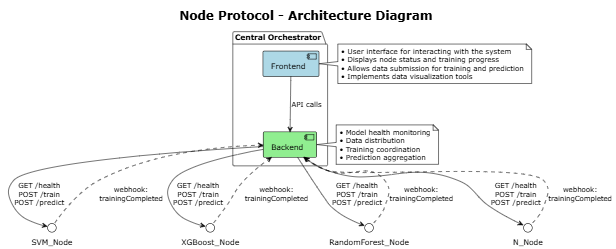
\includegraphics[width=\textwidth]{system-arch.png}
    \caption{Anomaly detection system design}
    \label{fig:system-design}
\end{figure}

\section{Outlier Protocol}

The outlier protocol is a custom protocol based on the OpenAPI specification. It is a simple protocol that describes how the orchestrator interacts with the model nodes, and is based on HTTP messages, which can be grouped into three main categories: \textit{health}, \textit{train}, and \textit{predict}.

The current implementation is based on offline data, and a preprocessing is required in order to transform real data to the model's accepted one. This preprocessing consists on triming the discharge data, removing data before the beginning of the experiment.

\subsection{Health}

Models must implement the \texttt{/health} endpoint in order to be visible to the orchestrator. The orchestrator will send a \texttt{GET} message at a variable time. If the model does not answer, orchestrator must consider the model as unavailable, and data must not be sent to this model.\ \autoref{fig:health-message} shows the sequence diagram of the health message and its response. This message also includes the model name, uptime, and last training time.

\begin{figure}[H]
    \centering
    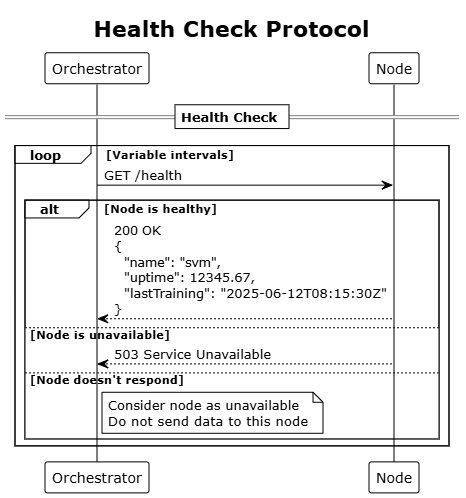
\includegraphics[width=0.75\textwidth]{health.png}
    \caption{Health message sequence diagram}
    \label{fig:health-message}
\end{figure}

\subsection{Train} 

This category describes how models will be trained in order to acquire data for disruption prediction. 

Protocol begins with a \texttt{post} message to the \texttt{/train} model endpoint that contains the number of discharges that will be sent to the models. Models that want to accept the training, answer with a 200 response. Then the orchestrator sends, one by one, the training discharges. After a discharge is received, models must acknowledge it. When all discharges are sent, models shall start the training.

When the training is done, models must inform the orchestrator, as shown in \autoref{fig:train-message}.

\begin{figure}[H]
    \centering
    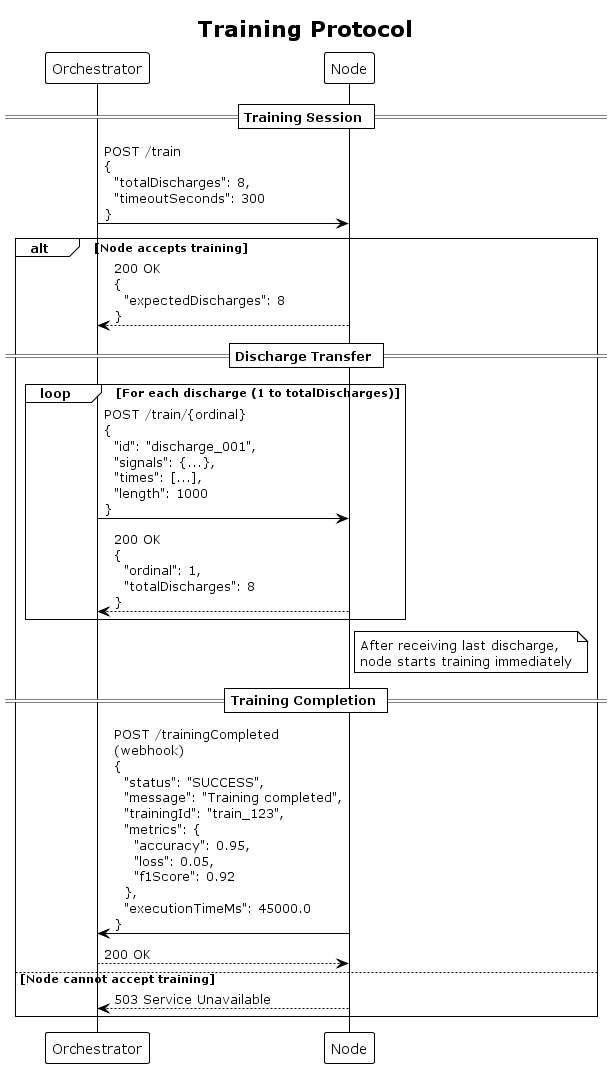
\includegraphics[width=0.75\textwidth]{train.png}
    \caption{Train message sequence diagram}
    \label{fig:train-message}
\end{figure}

\subsection{Predict}
\todo[inline]{Actualizar la figura de predict. En el outlier protocol no están puestas las features que se deben enviar.
\href{https://github.com/outlierClassifier/outlier_protocol/issues/3}{GH issue 3}}

The \texttt{predict} message is sent by the orchestrator to the alive models. It is a \texttt{POST} message to the \texttt{/predict} model endpoint and simulates online data. For this reason, models must send a prediction per window and the features that have been taken into account for the decision. Models must also report a \textit{justification} value, which is the confidence of that window to belong to a class.

\missingfigure{Prediction response message sequence diagram}

\section{Outlier Orchestrator}\label{sec:orchestrator}

The outlier orchestrator is the central node of the anomaly detection system. It is responsible for managing the data flow between the model nodes, using the outlier protocol to communicate with them.

The orchestrator consists on a frontend and a backend. The frontend is a web application that allows users to interact with the system, while the backend is responsible for managing the data flow and the communication with the model nodes.

The frontend is built using HTML, CSS, and JavaScript, and provides a user-friendly interface for managing the models and the data. It allows users to start and stop the models, view the health status of the models, and visualize the results of the anomaly detection.

The backend is built using Node.js, which is a JavaScript runtime that allows to run JavaScript code on the server side.

Communication between the frontend and the backend is done throw \texttt{Socket.io}, which is a library that allows real-time communication between the client and the server. This allows the frontend to receive updates from the backend in real-time, such as the health status of the models or the results of the anomaly detection.

\subsection{Frontend}

The frontend main page is shown in \autoref{fig:frontend-main}. There are two main panels: the top panel shows the available models, and the bottom panel consists on four tabs: \textit{Prediction}, \textit{Training}, \textit{History}, and \textit{Preview}.

\begin{figure}[H]
    \centering
    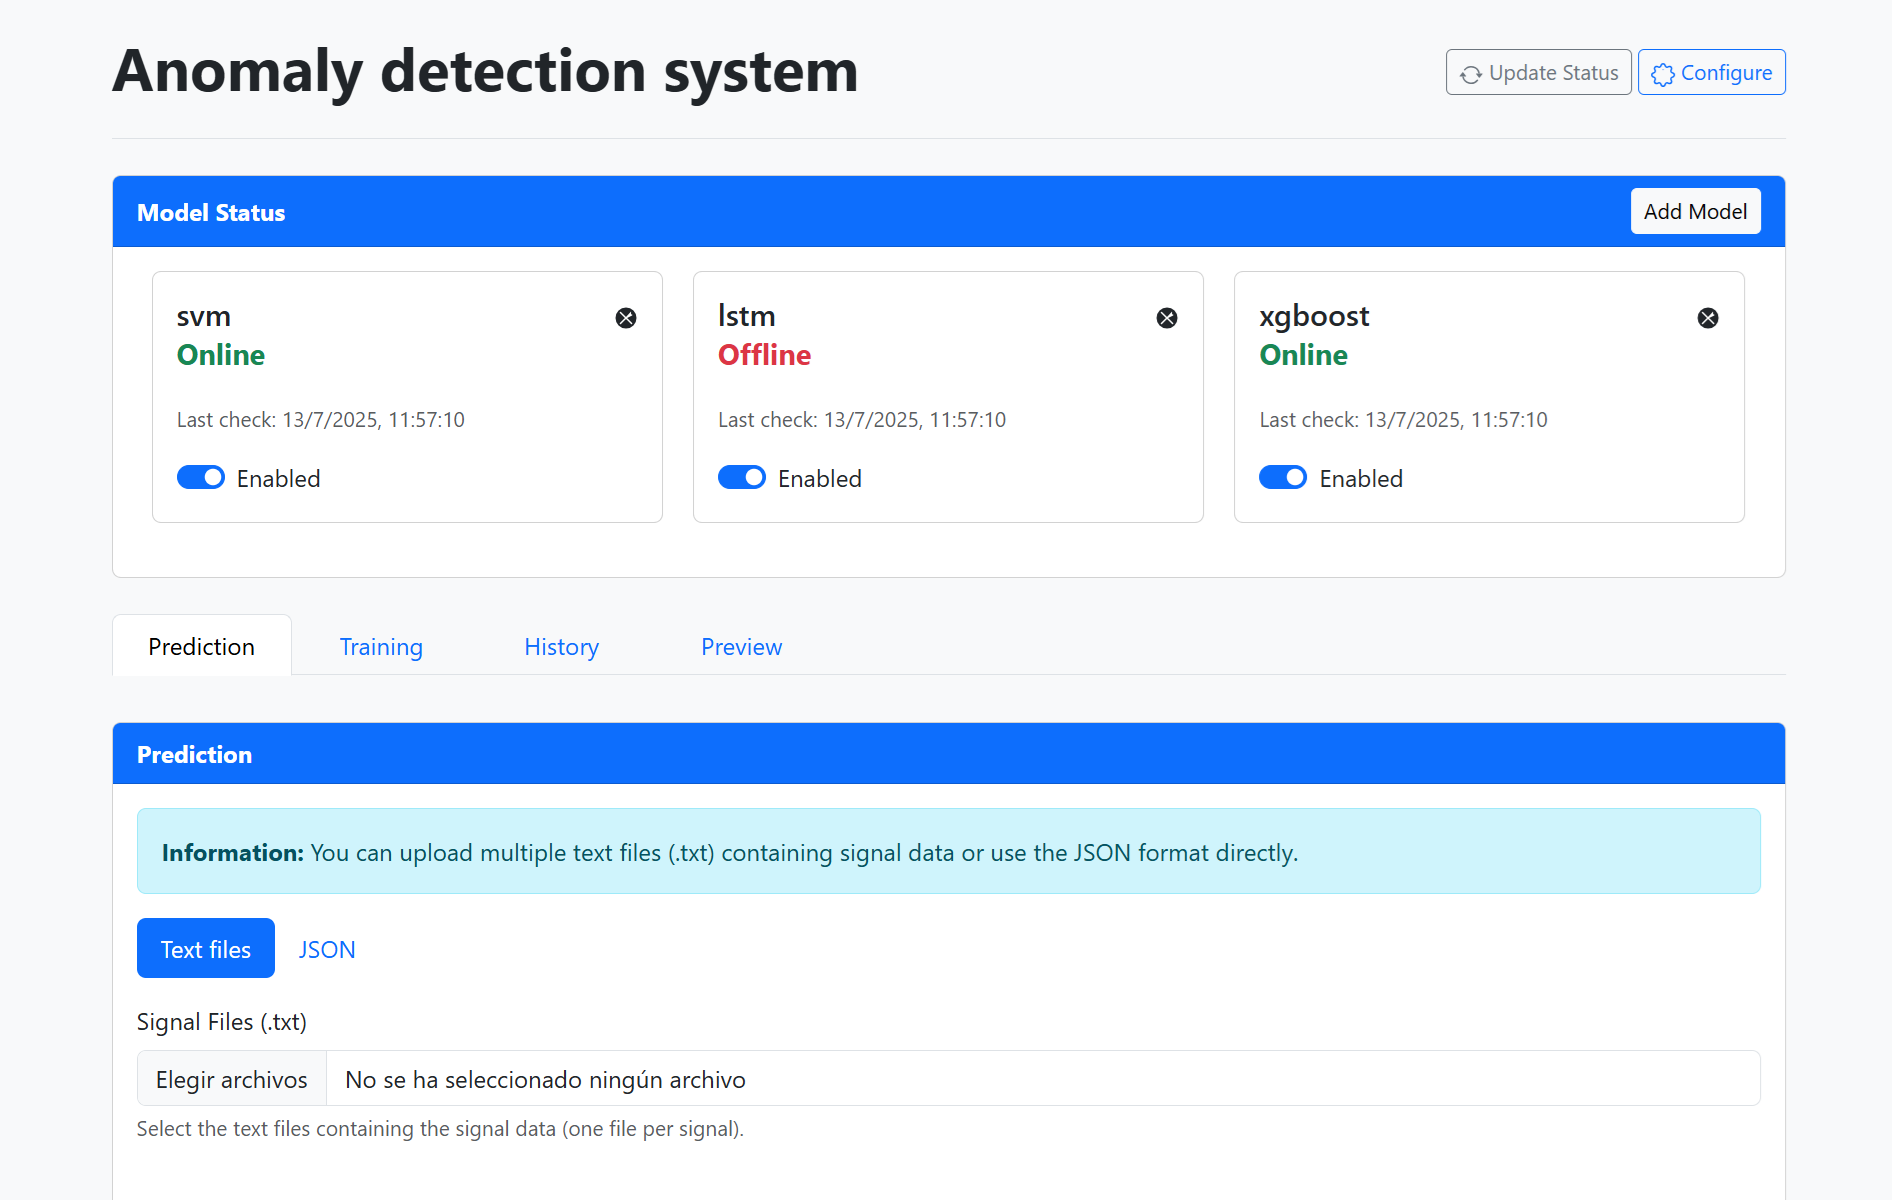
\includegraphics[width=\textwidth]{frontend-principal.png}
    \caption{Frontend main page}
    \label{fig:frontend-main}
\end{figure}

The backend is responsible for sending the model status to the frontend, including the health status, the training status and the prediction results, while the frontend is responsible of displaying this information to the user and sending the backend the user actions, such as adding or removing models, enabling or disabling models, changing model endpoints, starting a training, or making a prediction.

Model configuration is done through the \textit{Configure} button, which opens a modal where the user can change the model's endpoints. This modal is shown in \autoref{fig:frontend-configure}.

\begin{figure}[H]
    \centering
    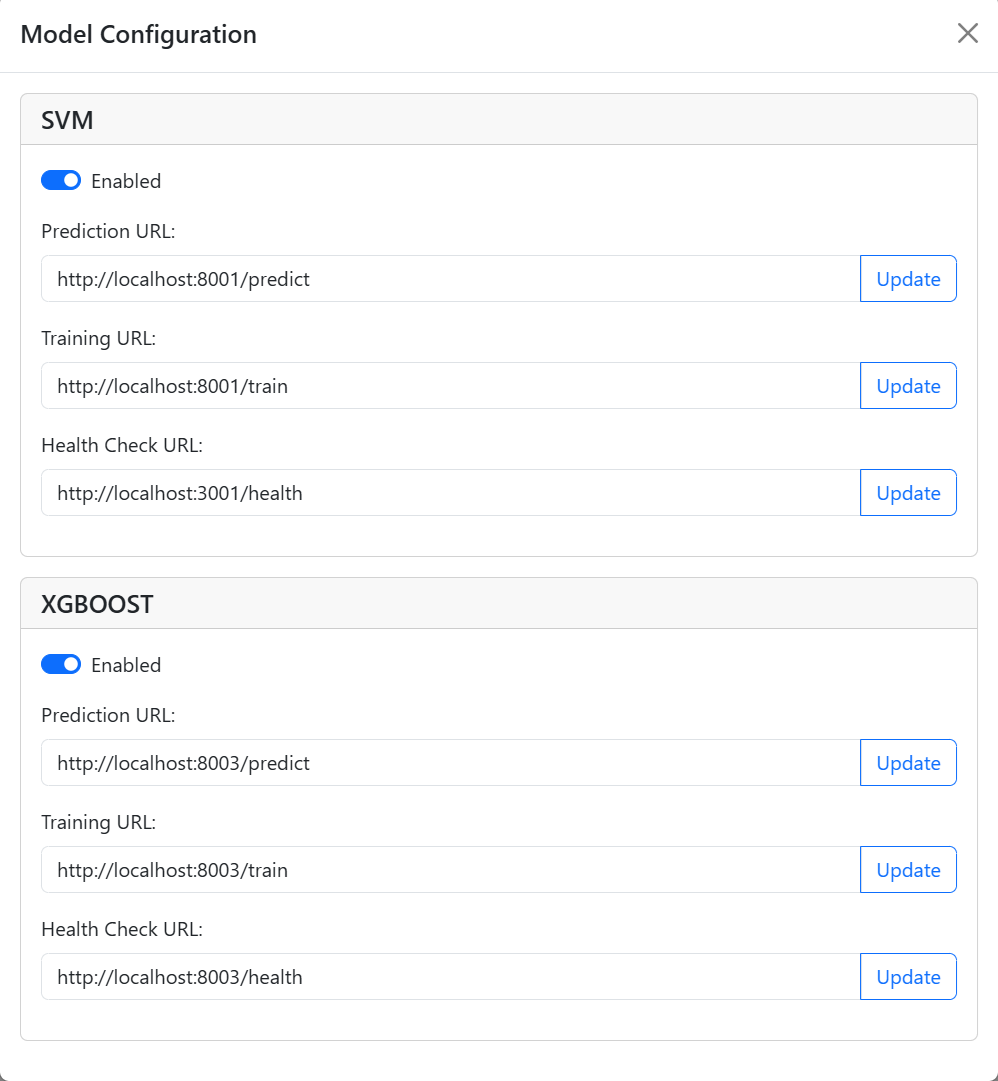
\includegraphics[width=0.5\textwidth]{model-configuration-modal.png}
    \caption{Model configuration modal}
    \label{fig:frontend-configure}
\end{figure}

\subsubsection{Prediction Tab}

The prediction tab allows users to make predictions using the available models. It provides a simple interface where users can choose the discharge to analyze. The \autoref{fig:frontend-prediction} shows the prediction tab and the result of a prediction.

\begin{figure}[H]
    \centering
    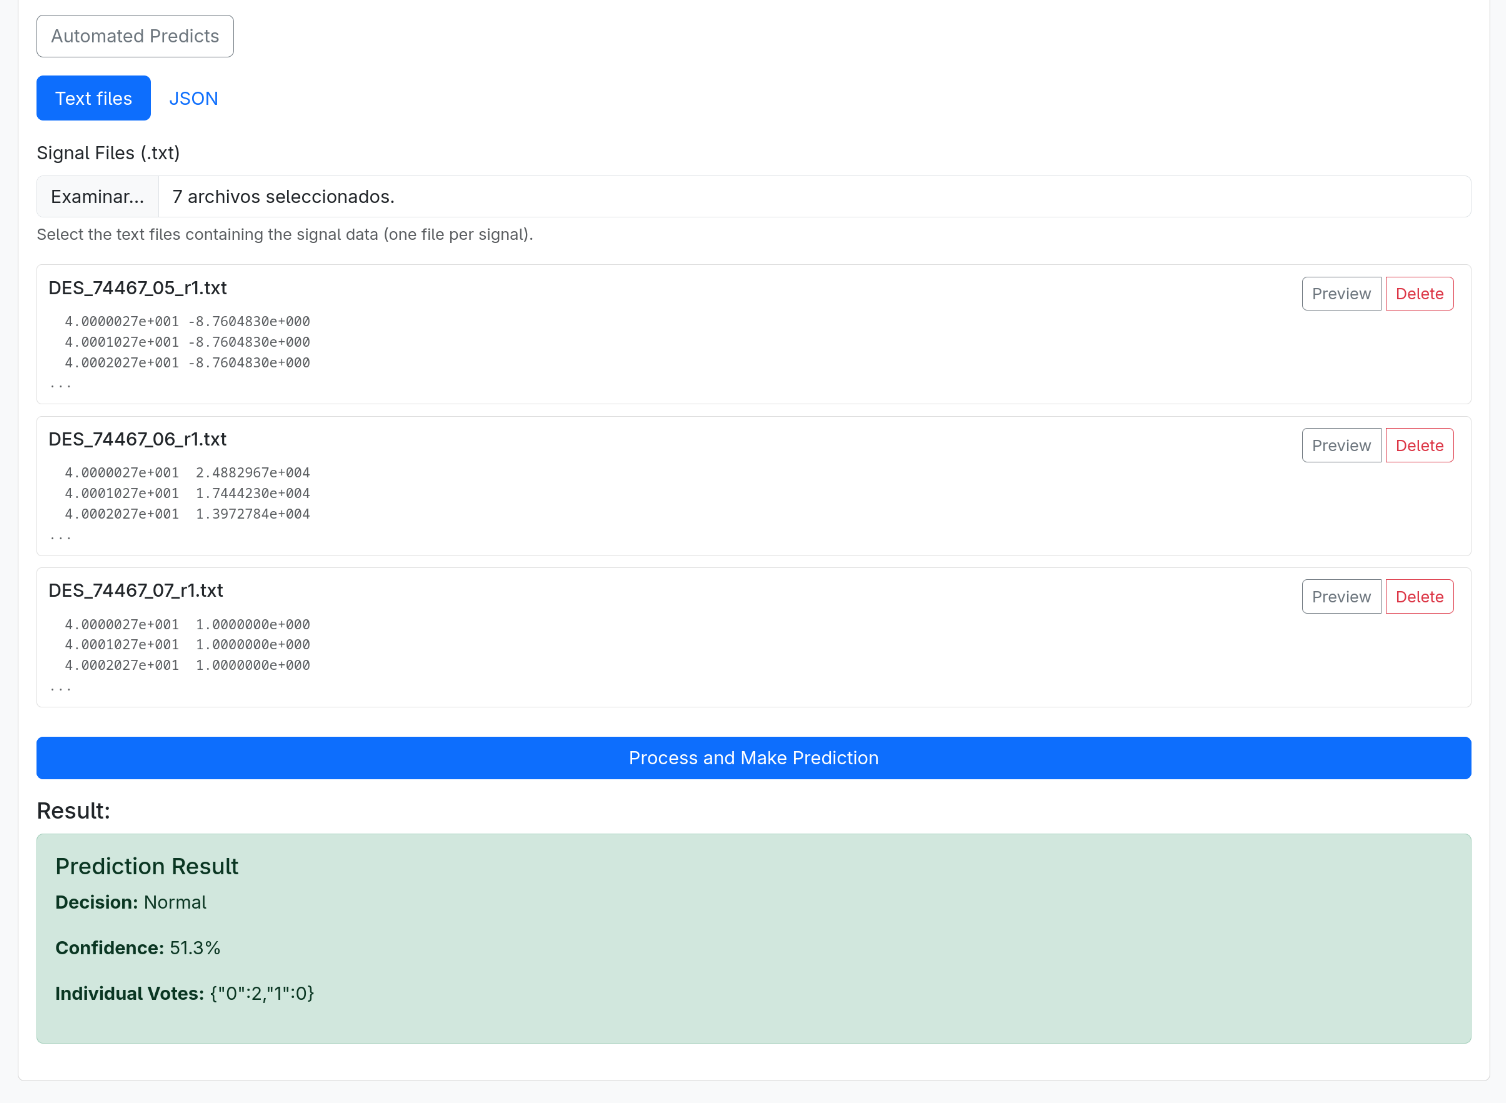
\includegraphics[width=\textwidth]{frontend-prediction.png}
    \caption{Frontend prediction tab}
    \label{fig:frontend-prediction}
\end{figure}

To ease models comparison, prediction orders can be automatically sent for discharges on a folder. As the Outlier Protocol specifies, models must report prediction per window, and add a justification. But models can differ in how do they calculate the final result. For example, as explained on \autoref{sec:models}, SVM calculates the distance to the separation hyperplane, and it is considered disruption if this value is positive, while XGBoost calculates a probability for being disruptive, so a value between 0 and 1 is returned. For this reason, user can set a threshold for a model, which is the first justification value that will be considered disruptive. Also, a \textit{count threshold} can be specified, this is, the number of consecutive windows that need to be labeled as disruptive to consider that discharge as disruptive. This behavior is represented on \autoref{fig:auto-pred}. The modal enables these personalization options for every online model. 

The frontend excludes the unwanted files and fetches the backend's \texttt{/api/ automated-predicts/session} endpoint, which handles user's information. On the backend section there is a detailed explanation of the implementation.

\begin{figure}[H]
    \centering
    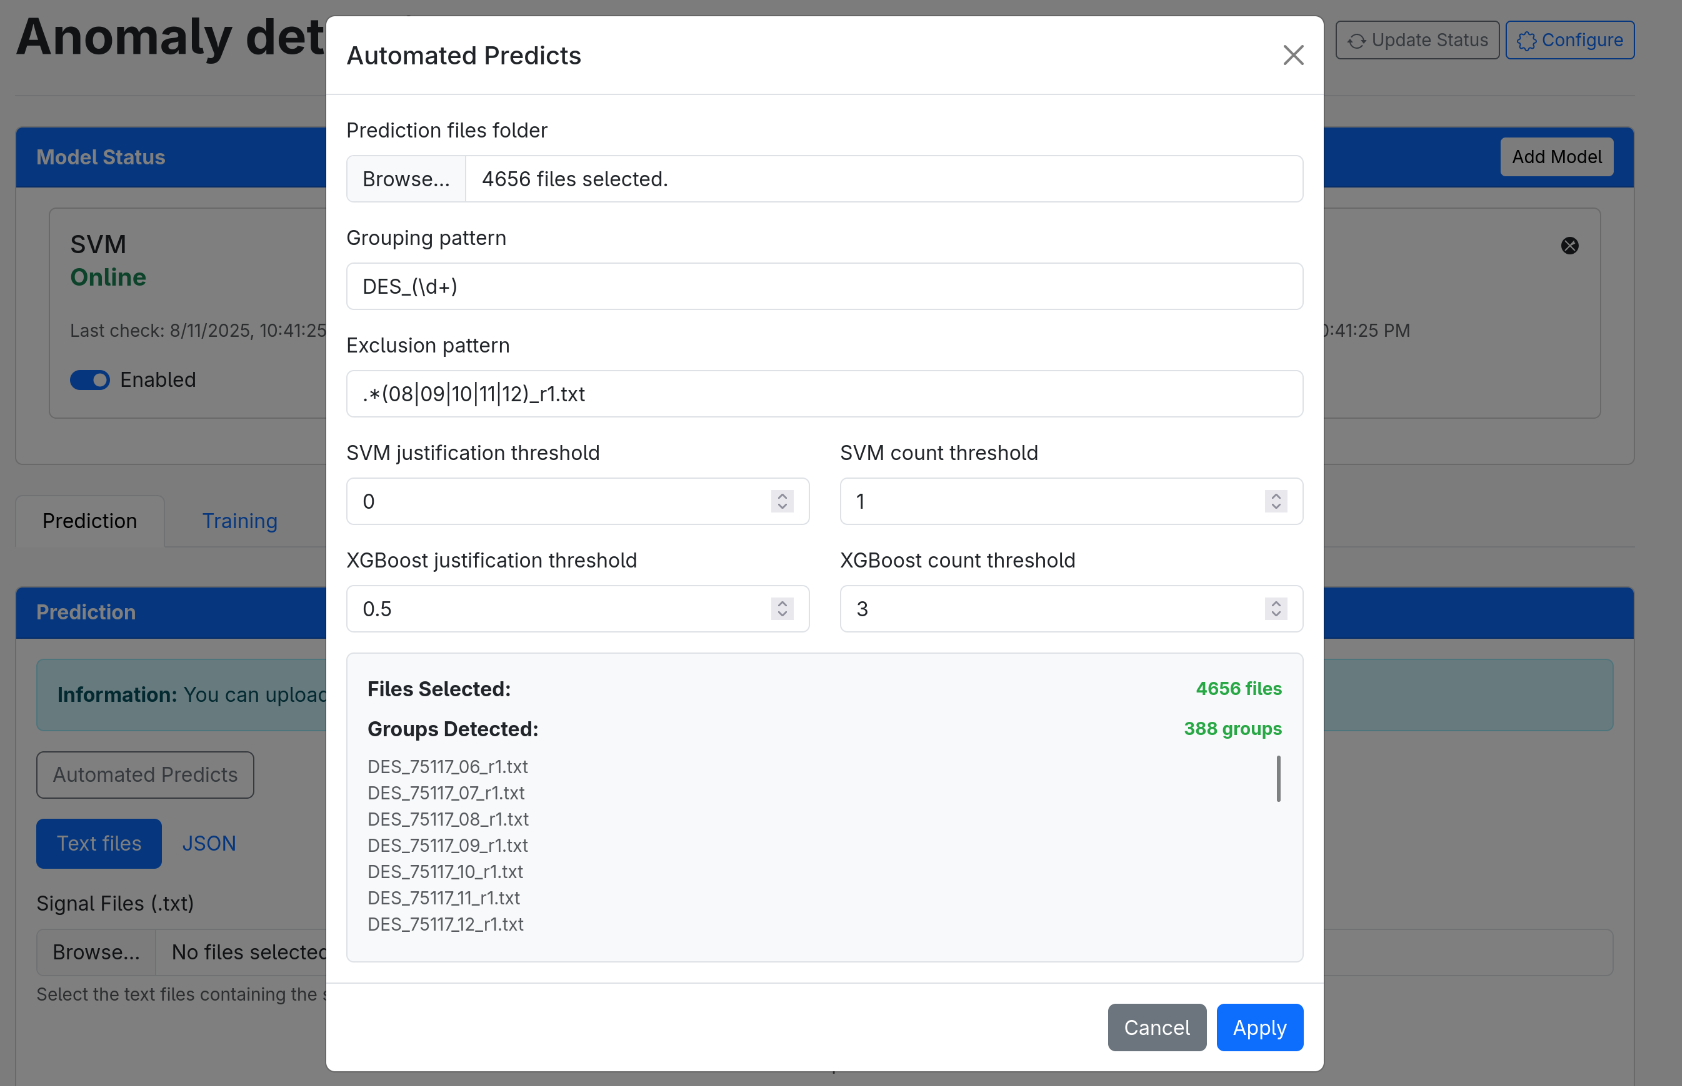
\includegraphics[width=\textwidth]{frontend-automated-predicts.png}
    \caption{Automated predictions}
    \label{fig:auto-pred}
\end{figure}

\subsubsection{Training Tab}

The training tab (\autoref{fig:frontend-training}) is similar to the prediction tab, but users shall select more than one discharge to train the models. For simplicity, there is a button that allow to add multiple discharges at once, opening a modal that allows to select multiple input files, group them using a custom regular expression, and exclude some files with another regular expression. This modal is shown in \autoref{fig:frontend-add-multiple-discharge}. Discharges can also be labeled as disruptive or non-disruptive by setting a disruption time.

\begin{figure}[H]
    \centering
    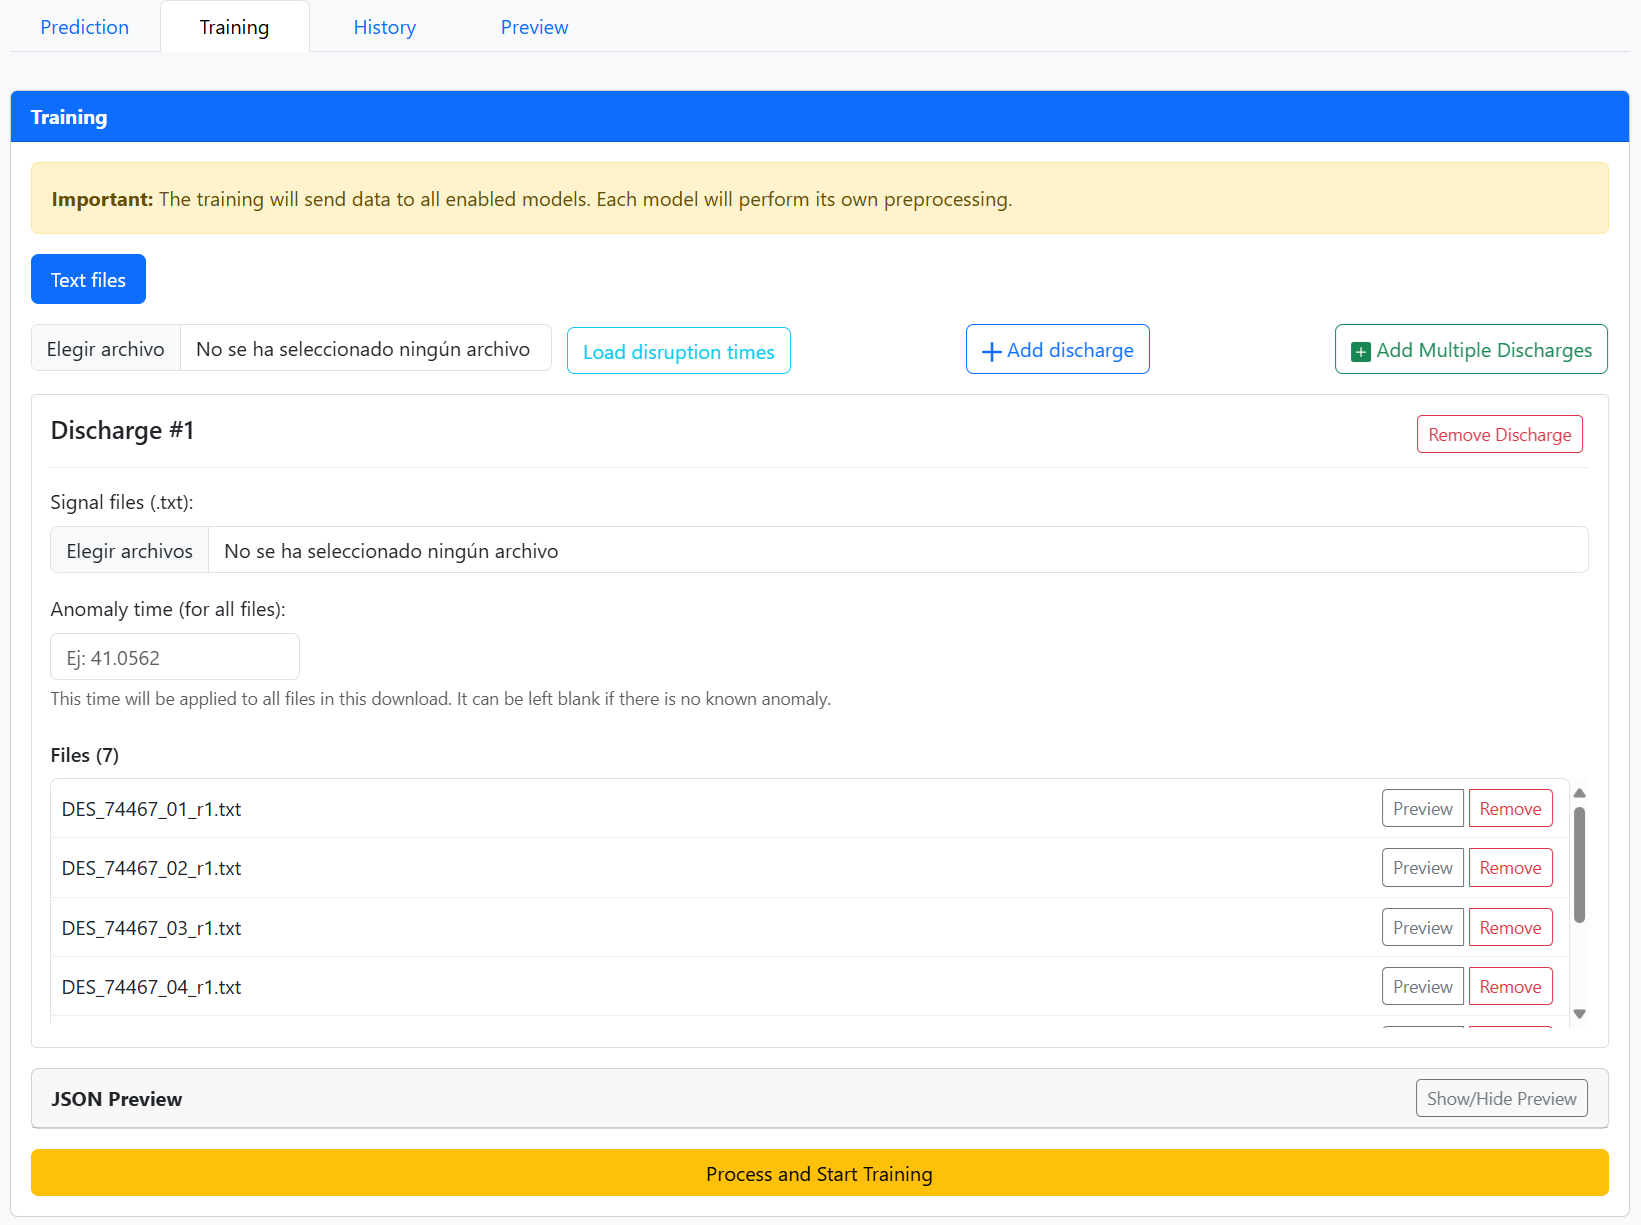
\includegraphics[width=\textwidth]{frontend-train.png}
    \caption{Frontend training tab}
    \label{fig:frontend-training}
\end{figure}

\begin{figure}[H]
    \centering
    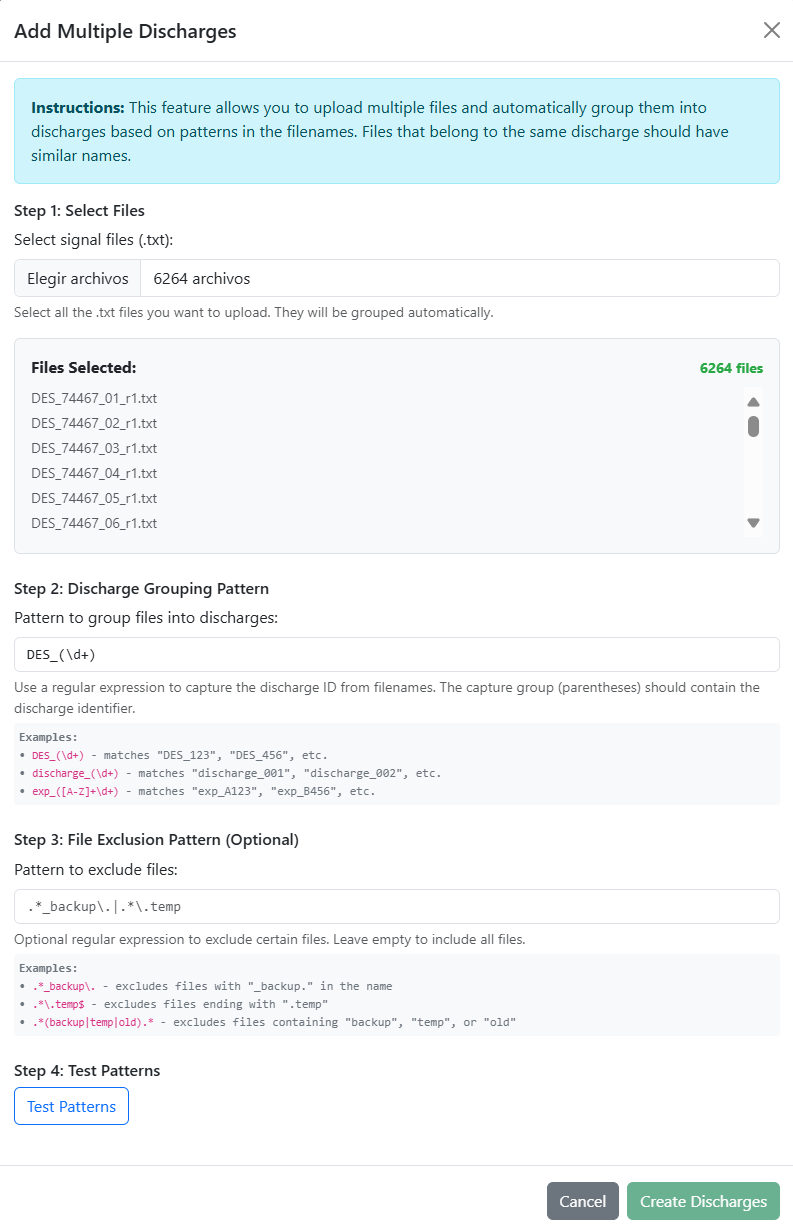
\includegraphics[width=0.5\textwidth]{multiple-discharge-modal.png}
    \caption{Add multiple discharges modal}
    \label{fig:frontend-add-multiple-discharge}
\end{figure}

\subsection{Backend}

The orchestrator's backend implementation is complex, as has to handle every possible message from the models. 

The orchestrator backend has three main components: the controller, the middleware and the services. 

The controller is a high-level class that stores model-related information, such as the current alive models, the prediction output, or the training process. It has advanced features for being efficient in memory usage, as queues to store just the necessary files while training. This feature is explained below.

The middleware is a group of utilities to validate input and output information. When the controller sends an order to the models, middleware ensures that information is well-formed to ensure compatibility. It also works on the other way, as model's messages are validated throw the middleware. This component guarantees that if an error occurs, it does not propagate and leads to undefined behavior.

The services component implements the low-level functionality that controller needs to communicate with the models, and exposes a high-level API that controller uses. This component includes the implementation of the voting mechanism, the batching feature to optimize memory usage or the training responses of models.

\subsubsection{Queuing and memory optimization}

The orchestrator is designed to handle multiple models and discharges simultaneously. As a training set can be large (thousands of discharges, each with thousands of windows), the orchestrator does not load every discharge into memory at once. Instead, one queue per model is created, where discharges are stored if needed, freeing memory when possible. The flow is as follows:

\begin{enumerate}
    \item User uploads training files in the dashboard interface through file input or drag-and-drop
    \item Frontend batches files into groups of 10 discharges to avoid overwhelming the server
    \item Frontend creates metadata containing total discharge count and batch discharge information
    \item Frontend sends an HTTP POST request to backend's \texttt{/api/train/raw} endpoint with the batch
    \item Controller receives batch and parses metadata to extract discharge information and file mappings
    \item Controller checks for existing training session or creates new one if none exists
    \item Controller starts a training session, which contacts all enabled models to initialize training
    \item Models respond with acceptance and each gets assigned a queue structure with sequence tracking
    \item Training session object is created with total discharge count, model queues, and processed discharge tracking
    \item Controller processes the current batch of discharges
    \item Service creates lazy stream generator that processes one discharge at a time from the batch
    \item Generator parses sensor files for each discharge individually, not loading all at once
    \item Each processed discharge added to all model queues simultaneously for parallel processing
    \item Discharge memory immediately released after being cloned to all model queues
    \item Asynchronous queue processors start for each model independently and concurrently
    \item Each model's queue processor sends discharges sequentially to that model's training endpoint
    \item Discharge memory released again after successful transmission to each model
    \item Queue processor continues until its queue is empty, then becomes idle
    \item Process repeats for each batch until all discharges sent
    \item Training session monitors progress and automatically finishes when total discharge count reached
    \item All queues emptied and training session cleaned up
    \item Models complete training and send completion notifications back to orchestrator.
\end{enumerate}


\subsubsection{Automated predicts and report generation}

As explained on the frontend section, to facilitate the prediction process, the orchestrator has a built-in feature that allows automatic predictions. This feature loads a directory and makes sequential predictions for each discharge. Orchestrator groups the files by a regular expression, and sends the discharges to the models one by one. Then, orchestrator stores the results and builds a report with statistical data. These results include raw outputs (prediction output per discharge), and a CSV grouping individual window predictions. Results are explained in \autoref{sec:cap4}.

\section{Outlier Models}\label{sec:models}

Every model node shall implement the outlier protocol in order to communicate with the orchestrator. This means that every model is a microservice implementing a server that exposes the necessary endpoints to the orchestrator. The models can be implemented in any programming language, as long as they can handle HTTP requests and responses. Models in this project are implemented in Python and Rust.

For compatibility reasons, every model must split discharges in windows of a fixed length (16 points per window). Models are allowed to extract any relevant data from the windows set.

\subsection{Supervised Binary Classification}

\subsubsection{\acs{SVM}: A Rust implementation of the \acs{APODIS} algorithm}\label{sec:svm-implementation}

This project implements the \ac{APODIS} algorithm for anomaly detection as a starting comparison point. The model is implemented in pure Rust, implementing the outlier protocol using the \texttt{actix\_server} framework for the communication with the orchestrator's backend, and the \texttt{linfa} crate for the \ac{SVM} implementation.

The feature extraction logic is implemented in the \texttt{get\_features} function, which extracts the mean and the standard deviation of the FFT magnitudes for each window. This function is shown in \autoref{lst:svm-features}.

\begin{lstlisting}[language=Rust, caption={Feature extraction for the \ac{SVM} model}, label={lst:svm-features}]
    fn get_features(
        &self, 
        window_size: usize
    ) -> (SignalFeatures, SignalFeatures) {
        let num_windows = self.values.len() / window_size;

        let mut mean_values = Vec::with_capacity(num_windows);
        let mut fft_std_values = Vec::with_capacity(num_windows);

        let mut planner = FftPlanner::new();
        let fft = planner.plan_fft_forward(window_size);

        for k in 0..num_windows {
            let start_idx = k * window_size;
            let end_idx = (k + 1) * window_size;
            let window = &self.values[start_idx..end_idx];

            let mean_value = window.iter().sum::<f64>() / window_size as f64;
            mean_values.push(mean_value);

            let mut fft_input: Vec<Complex<f64>> =
                window.iter().map(|&x| Complex::new(x, 0.0)).collect();

            fft.process(&mut fft_input);

            // Positive freqs (without DC component)
            // Only need up to window_size/2 due to symmetry
            let magnitudes: Vec<f64> = fft_input[1..=window_size / 2]
                .iter()
                .map(|c| c.norm())
                .collect();

            // std deviation of FFT magnitudes
            let fft_mean = magnitudes.iter().sum::<f64>() / magnitudes.len() as f64;
            let fft_variance = magnitudes
                .iter()
                .map(|&m| (m - fft_mean) * (m - fft_mean))
                .sum::<f64>() / magnitudes.len() as f64;

            let fft_std = fft_variance.sqrt();
            fft_std_values.push(fft_std);
        }

        (
            SignalFeatures {
                type_: FeatureType::Mean,
                values: mean_values,
            },
            SignalFeatures {
                type_: FeatureType::FftStd,
                values: fft_std_values,
            },
        )
    }
\end{lstlisting}

To train the model, SVM uses the \texttt{linfa} crate, which provides a high-level API for machine learning in Rust. The training process is done with the configuration which is shown in \autoref{lst:svm-train}. This function takes a dataset of features and labels, and trains the model using the \ac{SVM} algorithm with a Gaussian kernel.

\begin{lstlisting}[language=Rust, caption={Training the \ac{SVM} model}, label={lst:svm-train}]
    let model: Svm<f64, bool> = Svm::<f64, bool>::params()
        .gaussian_kernel(10.)
        .pos_neg_weights(1.0, 1.0)
        .fit(&dataset)
        .expect("Error training SVM model");
\end{lstlisting}

The prediction process is done for each window, and the model returns a boolean value indicating whether the window is anomalous or not. The prediction process is shown in \autoref{lst:svm-predict}. The model also returns the distance to the separation hyperplane, which is used to calculate the justification value.

\begin{lstlisting}[language=Rust, caption={Prediction with the \ac{SVM} model}, label={lst:svm-predict}]
    for (i, signal) in dataset
        .records
        .axis_iter(ndarray::Axis(0))
        .enumerate() 
    {
        let distance = model
            .as_ref()
            .unwrap()
            .weighted_sum(&signal.to_owned()) - model.as_ref().unwrap().rho;
        window_props.push(WindowProperties {
            feature_values: signal.to_vec(),
            prediction: if predictions[i] { 
                "Anomaly".to_string() 
                } else { "Normal".to_string() },
            distance,
        });
    }
\end{lstlisting}

It is important to note that the \ac{APODIS} algorithm does not specify which kernel to use, so the Gaussian kernel is used as a default. This kernel is a common choice for \ac{SVM} models, as it allows creating non-linear decision boundaries. But, as shown in \autoref{eq:svm-dual}, training consists on solving the dual problem, which is a quadratic programming problem. This means that training time is proportional to the number of discharges and the number of windows per discharge, which can lead to long training times for large datasets. With the available hardware for the project, it is not possible to train the model with all the C23 campaigns, as it would require 4.6376 Terabytes of RAM, which is not feasible. For this reason, model is trained with a subset of the discharges, which may lead to a loss of accuracy.

\subsubsection{XGBoost}\label{subsubsec:xgboost}

The XGBoost model is implemented in Python, using the \texttt{xgboost} library for the model, and the \texttt{fastapi} framework for the API.\ It is a supervised binary classification model that uses different features extracted from the discharges. These features include basic statics, like the mean and the mean of the slope of each window, the log of the \ac{RMS}, and dynamic features, like the maximum slope, and data related to the second derivative of each window (minimum, maximum and mean). In total, the model uses 7 features extracted from the discharge data for each window.

Model is also fed with the past features of the discharge, that are used as a tendency to give the model more context about the discharge. This means that the model needs a minimum number of windows to be able to make predictions, which is set to 3 windows by default. As past features are treated like the current features, the model uses a total of 28 features (7 features per window, and 4 windows). 

Feature extraction logic for the current window is implemented in the \texttt{extract\_ features} function, which is shown in \autoref{lst:xgboost-features}. This function takes a list of floats as input, which represents the discharge data for a window, and returns a numpy array with the extracted features. The function raises a \texttt{ValueError} if the input window is empty.\ \autoref{lst:xgboost-past-features} shows the feature extraction for the past windows, which is done by iterating over the past windows and extracting the features for each one. The features are then averaged to get a single feature vector for each past window.

\begin{lstlisting}[language=Python, caption={XGBoost feature extraction for the current window}, label={lst:xgboost-features}]
def extract_features(window: list[float]) -> np.ndarray:
    """Extract features from discharge data for model training/prediction"""

    if len(window) == 0:
        raise ValueError("Window cannot be empty")

    features = []

    mean = np.mean(window)
    if len(window) > 1:
        diff = np.diff(window)
    else:
        diff = np.array([0.0])

    if len(window) > 2:
        abs_second_derivate = np.abs(np.diff(diff))
    else:
        abs_second_derivate = np.array([0.0])

    features.extend([
        # Core statistics
        mean,
        diff.mean() * 1/SAMPLING_TIME, # Slope (mean of diffs) 
        np.log1p(np.sqrt(np.mean(np.square(window)))), # log of RMS

        # Dynamic features
        np.max(np.abs(diff)), # Max slope
        # Second derivative features
        np.min(abs_second_derivate) * 1/(SAMPLING_TIME**2),
        np.max(abs_second_derivate) * 1/(SAMPLING_TIME**2),
        np.mean(abs_second_derivate) * 1/(SAMPLING_TIME**2),
    ])
    return np.array(features).reshape(1, -1)
\end{lstlisting}

\begin{lstlisting}[language=Python, caption={XGBoost feature extraction for the past windows}, label={lst:xgboost-past-features}]
    for j in range(1, num_tendency + 1):
        prev_idx = window_idx - j
        if prev_idx in aligned_windows and len(aligned_windows[prev_idx]) > 0:
            prev_window_features = np.zeros(feature_size)
            for window in aligned_windows[prev_idx]:
                prev_window_features += extract_features(window)[0]
            prev_window_features /= len(aligned_windows[prev_idx])
            all_features.append(prev_window_features)
\end{lstlisting}

The necessary parameters to create an XGBoost model with the \texttt{xgboost} library are shown on \autoref{lst:xgboost-params}. These parameters are set to values that have been tested and work well for the project, but they can be modified to improve the model's performance. The \texttt{tree\_method} is set to \texttt{hist} to use a histogram-based algorithm, which is faster and more memory-efficient than the default \texttt{exact} method\todo{Ref}. The \texttt{n\_jobs} parameter is set to -1 to use all available CPU cores for training. The \texttt{objective} is set to \texttt{binary:logistic} for binary classification, and the evaluation metric is set to \texttt{aucpr} (area under the precision-recall curve) for better performance in imbalanced datasets, like the given ones.

\begin{lstlisting}[language=Python, caption={XGBoost model parameters}, label={lst:xgboost-params}]
    params = {
        # Algorithm and hardware settings
        'tree_method': 'hist',
        'n_jobs': -1,
        # Objective and evaluation metrics
        'objective': 'binary:logistic',
        'eval_metric': 'aucpr',
        # Regularization and overfitting control
        'learning_rate': 0.05,
        'scale_pos_weight': scale_pos_weight,
        # Hyperparameters
        'max_depth': 6,
        'min_child_weight': 3,
        'gamma': 1.0,
        'eta': 0.02,
        'subsample': 0.8,
        'colsample_bytree': 0.8,
    }

    dtrain = xgb.DMatrix(X_array, label=y_array)
    model = xgb.train(params, 
                      dtrain, 
                      num_boost_round=10000, 
                      verbose_eval=10
                      )

\end{lstlisting}

XGBoost predicts the probability of a window being disruptive, so a post-processing step is needed to determine if the discharge is disruptive or not. This post-processing step is done by the orchestrator, setting a threshold, which is set to 0.5 by default (50\% chance of being disruptive), and a number of consecutive windows that must be disruptive to consider the discharge as disruptive, which is set to 3 by default. This means that if 3 consecutive windows are above the threshold, the discharge is considered disruptive.

It is important to note that the XGBoost uses \texttt{scale\_pos\_weight} parameter to balance the classes. This means that the model is trained to give more importance to the disruptive class, as it is the minority class in the dataset. This parameter sets the weight of the positive class (disruptive) to the ratio of negative to positive samples, which is calculated as 

\begin{equation}
    w_i = \frac{N_{neg}}{N_{pos}}
    \label{eq:scale_pos_weight}
\end{equation}

This helps the model to learn better from the minority class and improve its performance. This value is approximately 11 for the C23 campaign, as there are 11 non-disruptive windows for each disruptive window.

\subsubsection{CNN-FFT}

\subsection{Outlier Detection}

This section explains outlier detection models that are implemented for the project. These models are only trained with non-disruptive discharges, and try to find common patterns between them. If a window differs more than a threshold from the pattern, it is labeled as disruptive.

\subsubsection{\acs{OC-SVM}}

\subsubsection{Isolation Forest}

The \ac{IForest} model is implemented in Python, using \texttt{sklearn} library for the model, and the \texttt{fastapi} framework for the API.\ As \texttt{sklearn} is used, if a \ac{GPU} is available, it will be used to improve training times.

The feature extraction logic differs from other models. As this is a non supervised model, a rich set of features is used to enhance the model's performance. Basic statistics are extracted, like the mean and the standard deviation of each window, but also inter-signal features, like the ratio of the radiated power to the plasma current, the Greenwald density fraction, the locked mode norm, the inner inductance norm, and the beta loss.


\begin{lstlisting}[language=Python, caption={Inter-signal features extraction}, label={lst:inter-signal-features}]
for w_idx in range(n_windows):
    mean_vals = [float(np.mean(sig.values[start:end])) for sig in discharge.signals]

    Ip_MA = mean_vals[0] * 1e-6
    n_1e20 = mean_vals[3] * 1e-20

    # Inter signal features.
    A_MINOR = 0.95 / 2.0  # Minor radius of the JET tokamak in meters. Used in the Greenwald limit.
    rad_power_ratio = mean_vals[5] / mean_vals[6] if mean_vals[6] != 0.0 else 0.0
    greenwald_density_frac = n_1e20 / (Ip_MA / (np.pi * A_MINOR**2)) if Ip_MA != 0.0 else 0.0
    locked_mode_norm = mean_vals[1] / Ip_MA if Ip_MA != 0.0 else 0.0
    inner_induct_norm = mean_vals[2] / Ip_MA if Ip_MA != 0.0 else 0.0
    beta_loss = abs(mean_vals[5]) / mean_vals[6] if mean_vals[6] != 0.0 else 0.0

    inter_features = [
        rad_power_ratio, greenwald_density_frac,
        locked_mode_norm, inner_induct_norm, beta_loss
    ]
\end{lstlisting}

\subsubsection{\acs{LSTM}}


\chapter{Budget} \label{sec:cap4}

\chapter{Impact} \label{sec:cap5}

%En este capítulo el estudiante pondrá de manifiesto las implicaciones sociales, de salud y seguridad, ambientales, económicas, tecnológicas o industriales que estén relacionadas son su trabajo, así como la posible aportación a los ODS (Objetivos de Desarrollo Sostenible.

% Referencias útiles para elaborar este capítulo:
% \begin{itemize}
%     \item Naciones Unidas. Objetivos de Desarrollo Sostenible. Online: https://www.un.org/sustainabledevelopment/es/objetivos-de-desarrollo-sostenible/
%     \item Fernández Aller, Celia; Miñano, Rafael. "Guía para trabajar la Responsabilidad Social y Ambiental (GRSA)". ETSI Sistemas Informáticos, UPM. (Versión 2.0 Mayo 2015). Online: 
    
%     \href{https://oa.upm.es/35542/1/Guia_Responsabilidad_Social_y_Ambiental-V2-1.pdf}{https://oa.upm.es/35542/1/Guia\_Responsabilidad\_Social\_y\_Ambiental-V2-1.pdf}
%     \begin{itemize}
%         \item Páginas especialmente útiles para estudiantes de PFG: 31 a 40.
%     \end{itemize}
% \end{itemize}



% Conclusiones (obligatorio)
\chapter{Conclusions and future work} \label{sec:cap6}
% \noindent En el último apartado de la memoria se ha de incluir una visión general del trabajo realizado: problema propuesto, solución planteada y resultados obtenidos. Junto con esta descripción, también hay que especificar qué conocimiento nuevo se puede derivar de toda la información expuesta en el informe: validez o no del sistema, nuevos aspectos del problema detectados en el trabajo, etc. Finalmente, si el proyecto no deja totalmente cerrado y resuelto el problema tecnológico abordado, el proyectista debe aprovechar su experiencia para proponer líneas futuras de trabajo.


\label{sec:bibliografía}
\printbibliography

% Anexo (obligatorio)
\appendix
\label{sec:apendice}

\end{document}